\documentclass[10pt,a4paper]{article}
\usepackage[T1]{fontenc}
\usepackage[utf8]{inputenc}
\usepackage{lmodern,graphicx,booktabs,longtable,array,amsmath,amssymb,float}
\usepackage[margin=18mm]{geometry}
\usepackage[numbers,sort&compress]{natbib}
\usepackage[hyphens]{url}
\usepackage[hidelinks]{hyperref}
\IfFileExists{microtype.sty}{\usepackage{microtype}}{}
\IfFileExists{caption.sty}{\usepackage[font=small,labelfont=bf]{caption}}{}
\setlength{\parskip}{4pt}
\setlength{\parindent}{0pt}
\setlength{\emergencystretch}{3em}
\setlength{\textfloatsep}{12pt}
\setlength{\intextsep}{12pt}
\setlength{\abovecaptionskip}{6pt}
\renewcommand{\topfraction}{.92}
\renewcommand{\bottomfraction}{.88}
\renewcommand{\textfraction}{.06}
\renewcommand{\floatpagefraction}{.82}
\widowpenalty=10000
\clubpenalty=10000
\makeatletter
\setlength{\@fptop}{0pt}
\makeatother
\newcommand{\figref}[1]{Fig.~\ref{fig:#1}}
\title{Supplementary information: A common BSA--serum equation for EASI estimation in a Chinese atopic dermatitis cohort}
\author{}
\date{}
\begin{document}
\maketitle
\renewcommand{\thetable}{S\arabic{table}}
\renewcommand{\theHtable}{S.\arabic{table}}
\section*{Supplementary guide}
The Supplementary Methods define the analysis populations, endpoints and validation. Tables S1--S5 provide exact target rates, complete model metrics, safety-documentation coverage, reference-exclusion sensitivity and input/reference specifications. Figures are grouped by their clinical or measurement question below. Complete aggregate results, including negative and non-estimable findings, remain in the linked CSV collection. Missing estimates are not zero effects.
\hyperref[fig:FigureS1]{\textbf{Cohort structure and treatment comparability}}. Clinical and model eligibility, baseline balance and common treatment support.\par
\hyperref[fig:FigureS3]{\textbf{Clinical outcomes and target comparisons}}. Observed and adjusted clinical scores, laboratory follow-up and all specified treatment contrasts.\par
\hyperref[fig:FigureS11]{\textbf{Serum changes and regional disease}}. The complete23-marker panel, paired treatment windows, clinical associations and regional burden.\par
\hyperref[fig:FigureS20]{\textbf{Individual EASI estimation and monitoring}}. Absolute-score agreement, baseline severity, paired changes and response classification.\par
D denotes dupilumab; A100/A200 denote initial abrocitinib 100/200 mg. Treatment colours are fixed throughout. Molecular changes use log$_2$ concentration units; a change of $-1$ means a halving. Model errors use EASI points. Correlation describes ordering, whereas absolute errors and concordance address numerical agreement.
\clearpage
\section{Supplementary Methods}
\subsection{Study design and clinical records}
This analysis used longitudinal records from a Chinese observational treat-to-target project. The supplied protocol specified clinician-directed systemic treatment rather than random allocation. We retained the initial treatment group for longitudinal comparisons and separately extracted subsequent dose, interval, stopping, switching and restart information. The analysed records came from CAMS and Huashan. The protocol's planned centre list and planned sample size were not substituted for the observed cohort.

The clinical dose-comparison population included patients aged at least 12 years with a known initial regimen. Six of 170 source patients were below age 12 and one had an unresolved initial dose, leaving 163 patients (65/56/42 by initial treatment). Records with unresolved simultaneous initial-dose assignments were excluded from dose-specific comparisons but retained in the source audit. Adult DLQI analyses used age at least 18. Baseline Table 1 uses one observed W0 record per eligible patient, with no weighting or imputation. Continuous summaries use median and quartiles with linear interpolation, rank $1+(n-1)p$ (type 7; Excel PERCENTILE.INC); all available denominators are reported. Age and BMI are also presented as medians, rather than means and standard deviations. Repeated records were linked by the study patient identifier and nominal visit; a patient was never treated as a new independent person at each visit. The requested reporting visits were W0, W2, W4, W12 and W24 for PP-NRS; W0, W4, W12 and W24 for EASI, IGA, DLQI, BSA, SCORAD and eosinophils; and W0, W12 and W24 for IgE. Low-coverage intermediate visits were retained in the underlying data but were not inserted into these trajectories.

EASI was the recorded clinical reference outcome. Source discrepancies between regional sums and total EASI were audited rather than silently repaired. IGA grades were retained as recorded, including grade 5. Confirmation of the exact IGA version and PP-NRS recall window remains necessary. Nominal clinical/serum visit linkage does not by itself verify that the blood draw and examination occurred on the same calendar day; exact dates and a permissible matching window require source confirmation. Among the 152/89/75 model visits at W0/W12/W24, 8/2/0 had complete regional scores whose sum differed from total EASI by more than 0.15; the largest absolute gaps were 18.7/8.5/0.0 points, and 1/1/4 visits lacked a complete regional reference. Restricting evaluation to all four regions observed with total--sum difference at most 0.01 retained 140/86/71 visits and gave MAEs 3.17/1.32/1.11. This evaluation-only sensitivity uses unchanged saved predictions. A separate training-exclusion sensitivity removed the eight W0 and two W12 discrepant visits from fitting, retained missing-region visits, and repeated preprocessing and inner structure/penalty selection within the original patient folds. Evaluation patients and recorded outcomes were unchanged. It gave W0/W12/W24 MAEs of 3.19/1.15/1.06; matched BSA controls were refitted identically. Neither analysis adjudicates which clinical reference is correct (Supplementary Table~\ref{tab:reference_sensitivity}). Details are in \texttt{model\_reference\_QC\_audit.csv}.

\subsection{Clinical targets and treatment comparisons}
The week-2 target was PP-NRS $\leq4$. At week 4, the physician domain was EASI50 or an IGA decrease of at least two points, and the patient domain was PP-NRS $\leq4$ or adult DLQI $\leq10$. At week 12, the physician domain was EASI75 or IGA 0/1, and the patient domain was PP-NRS 0/1 or adult DLQI $\leq4$. At week 24, EASI $\leq5$ was an additional physician-domain criterion. The combined target required both domains. Because instrument identity and recall windows remain unresolved, these are exploratory targets based on the recorded scores. These are the investigators' operational definitions; they were not retrospectively relabelled as the newer IEC low-disease-activity or remission definitions.\citep{merola2026iec}

For an OR criterion, one observed positive component established success; a negative result required all components to be observed and negative. For an AND criterion, one observed negative component established failure; success required both positive components. Other cases remained unknown. Adult DLQI was an unknown component for ages 12--17, not a negative component and not removed from the OR rule. Thus adolescent itch success establishes the patient target; itch failure alone does not establish patient-target failure. The audit exhaustively verified the nine two-component truth states and reconciled every saved composite. Among 15 adolescents, the patient domain had 6/0/9 successes/failures/unknowns at W4, 4/0/11 at W12 and 4/0/11 at W24; the combined domain had 5/1/9, 4/5/6 and 4/3/8. An explicitly different PP-NRS-only adolescent rule would make five W12 and four W24 patient-domain unknowns determinate, including one W24 combined outcome. This is a sensitivity count, not a redefinition of the primary composite. Age-stratified counts are in \texttt{composite\_age\_evaluability\_audit.csv}. EASI response required an observed positive baseline. Individual thresholds were also analysed separately. Proportions used endpoint-specific observed denominators and Wilson 95\% confidence intervals. Overall three-group tests used conditional Monte Carlo Pearson tests with 49,999 draws, and pairwise comparisons used Fisher's exact test and risk-difference intervals. The three pairwise comparisons within an endpoint and visit formed a Holm family; exploratory FDR results were also retained. Overall tests were not included as an extra member of that pairwise family.

Baseline-adjusted binary target rates and risk differences used generalized overlap weights from a multinomial initial-treatment model with baseline EASI, age, sex, BMI and centre. We used 1,000 patient bootstrap resamples, stratified by initial treatment and refitting the propensity model, for percentile intervals. Two-sided P values used normal Wald tests based on bootstrap standard errors; three-group tests used a two-degree-of-freedom Wald statistic. The three individual pairwise comparisons formed a Holm family. Weighted results supplement the observed numerator and denominator. The primary target analysis used bootstrap seed 20261017. A revision W2 sensitivity added baseline PP-NRS to the propensity model. One patient lacked baseline PP-NRS; both the original-covariate model and the added-itch model were fitted on the remaining 162 patients, with the original 163-patient analysis retained. The same standardized logistic model (ridge parameter $C=1$), 1,000 stratified patient resamples and seed 20261018 were used for this sensitivity. The revision files also contain a separate full-cohort run with seed 20261018. Its point estimates use the same analysis, but its Monte Carlo intervals and Wald P values are not the frozen primary results; borderline changes were not selected for the main claim. The added-itch 100 mg--dupilumab contrast was 41.4 percentage points (95\% CI, 13.0--66.8; three-contrast Holm $P=0.0104$); the 100-minus-200 mg contrast was 6.7 points ($-11.3$ to 26.2). The largest endpoint-specific absolute standardized difference was 0.53 even after adding itch, so residual imbalance remained. Baseline weights were retained when calculating available-case balance and ESS; no claim of balanced follow-up selection is made. The table below reports both unweighted and matching baseline-overlap-weighted worst/best bounds, assigning every unknown outcome failure/success while retaining baseline weights. These bound the initial cohort under extreme missing-outcome assignments; the reported weighted available-case rate represents patients with that endpoint observed. Endpoint-specific overlap-weight ESS is reported separately. Bounds are sensitivity limits, not confidence intervals.
\begin{center}\small\textbf{Unweighted observed outcomes and initial-cohort bounds}\par\smallskip\begin{tabular}{llrrrr}\toprule Target & Initial group & Success/evaluable & Initial N & \shortstack{Observed\\rate, \%} & \shortstack{Unweighted missing-\\outcome bounds, \%} \\ \midrule
W2 itch & dupi & 15/27 & 65 & 55.6 & 23.1--81.5 \\
W2 itch & abro 100 mg & 34/37 & 56 & 91.9 & 60.7--94.6 \\
W2 itch & abro 200 mg & 33/36 & 42 & 91.7 & 78.6--92.9 \\
W24 combined & dupi & 26/36 & 65 & 72.2 & 40.0--84.6 \\
W24 combined & abro 100 mg & 22/24 & 56 & 91.7 & 39.3--96.4 \\
W24 combined & abro 200 mg & 20/23 & 42 & 87.0 & 47.6--92.9 \\
\bottomrule\end{tabular}\par\medskip\textbf{Matching baseline-overlap-weighted analysis}\par\smallskip\begin{tabular}{llrrr}\toprule Target & Initial group & \shortstack{Weighted available-\\case rate, \%} & \shortstack{Available-case\\weight ESS} & \shortstack{Weighted missing-\\outcome bounds, \%} \\ \midrule
W2 itch & dupi & 51.9 & 17.6 & 19.4--82.0 \\
W2 itch & abro 100 mg & 93.6 & 25.1 & 76.0--94.8 \\
W2 itch & abro 200 mg & 85.8 & 21.1 & 63.3--89.5 \\
W24 combined & dupi & 46.2 & 20.8 & 22.0--74.3 \\
W24 combined & abro 100 mg & 85.4 & 14.7 & 26.2--95.5 \\
W24 combined & abro 200 mg & 87.0 & 12.5 & 38.3--94.3 \\
\bottomrule\end{tabular}
\par\smallskip\parbox{.97\linewidth}{\footnotesize Bounds assign all unknown outcomes failure or success in the initial cohort. Weighted bounds retain the same baseline overlap weights in observed and unknown records. Weighted available-case rates use only endpoint-observed patients. ESS is the effective sample size of those weighted available cases, not a patient count or an incidence denominator. Bounds are sensitivity limits, not confidence intervals.}
\end{center}
 For generalized propensity scores $e_t(x)$, the weight is $h(x)/e_t(x)$, with $h(x)=1/\sum_t[1/e_t(x)]$. The baseline weighting function defines a common treatment-overlap population; an available-outcome analysis can depart from that population through selective observation. Covariate balance, propensity distributions and analysis-specific effective sample sizes are reported; weighting does not establish elimination of confounding.\citep{lili2019}

Continuous treatment comparisons used marginal regression with baseline outcome, treatment-by-visit terms, age, sex, BMI and centre. Generalized overlap weights addressed measured baseline differences in initial treatment selection. Patient-cluster robust covariance accounted for repeated outcomes, and a singular-value decomposition check prevented reporting non-estimable treatment-by-visit cells. IgE and eosinophils used log$(1+x)$; back-transformed estimates are not arithmetic means. No dupilumab W4 eosinophil measurements were available. That treatment-by-visit cell was not estimable without additional cross-treatment or temporal restrictions, so it remained blank. Multiple imputation would require unsupported assumptions about that unobserved cell and was not used to complete the observed trajectory. The fixed-patient IgE display uses the same patients at W0/W12/W24; adjusted comparisons are shown separately from raw medians. Unweighted adjustment, group balance, observation patterns and supplementary dupilumab-versus-pooled-abrocitinib contrasts were retained. Pooling used the observed dose mixture and did not erase the two initial abrocitinib groups. The comparisons estimate adjusted observational associations, not randomized fixed-dose effects. Nominal eligibility based on the registry filename date placed all initial patients beyond W24, but this administrative sensitivity is not an approved database lock or verified visit window. Reasons for absent assessments were unavailable.

Treatment reductions were assigned from recorded regimen intervals, with assessment/decision ordering marked uncertain at shared visit boundaries. A later reduction was not moved to an earlier visit. W12 response and subsequent regimen changes defined descriptive maintenance pathways. Analyses used observed W24 EASI75, explicit missing-outcome bounds and fixed-patient trajectories where all three visits were observed. This approach distinguishes treatment initiation from the selected maintenance pathways, consistent with the need to specify how intercurrent treatment changes enter the question being estimated.\citep{iche9r1} It does not identify a counterfactual outcome under a different regimen. At W0, two source records labelled initial 100 mg explicitly listed a 200 mg starting regimen, and one labelled initial 200 mg listed 100 mg. These are conflicts between the source group and regimen fields, not demonstrated post-baseline switches. The group labels were retained, and \texttt{exposure\_W0\_source\_adjudication.csv} preserves their counts separately from unknown exposure. Clinical-record adjudication is still required.

\subsection{Serum measurements and molecular analyses}
The laboratory source reports identify serum samples analysed with Luminex and MSD platforms. Luminex used an R\&D Systems LXSAHM-13 panel and Luminex-200; the MSD reports identify K15067M-1/K15067M-2 kits and an SQ120 instrument. Reports describe 50-$\mu$L serum and twofold dilution. The service-batch sample count was not used as the study sample size. Assay lots, run identifiers and source links remain in the restricted provenance records.

The analysis used the numeric integration export rather than the vendor's filtered display matrix. Positive export numerics recorded in pg/mL were log$_2$ transformed once, unchanged; the analysis applied no additional twofold dilution correction. This reproduces the fitted scale rather than verifying how the laboratory corrected its export for dilution. Explicit censoring strings and nonpositive values were not converted to measured positive concentrations. The vendor's filtered output can replace values below range with zero and values above range with an upper bound; those conventions must not be interpreted as exact measured concentrations. A sensitivity analysis represented IL-5 values below twice the software calibration lower bound at that boundary and repeated the model workflow. The software boundary is not an independently validated clinical quantification limit. Cross-platform bridging, technical-repeat precision and lot effects require additional assay documentation.

All 23 measured markers were retained. Molecular changes were formed within each patient and visit pair before group summaries, avoiding subtraction of averages from different patient sets. We analysed W0--W12, W12--W24 and W0--W24 separately. Mean log$_2$ changes were accompanied by t-based confidence intervals when at least five pairs were available. Smaller sets were descriptive. Two-sided paired mean-change sign-flip tests retained zero changes and ties. They enumerated all $2^n$ signs when $n\leq15$; otherwise they used 19,999 random signs (seed 20261002), counting exceedances at the observed absolute mean with a plus-one numerator and denominator. All-zero changes gave $P=1$. The sign-flip null assumes independent patients and sign-exchangeable paired changes (symmetry about zero); it is not a randomized-treatment test. Benjamini--Hochberg adjustment covered the full 23-marker, three-treatment, three-window family: 207 planned cells, of which 193 had estimable P values. Non-estimable cells remained missing and were not counted as tests. Between-treatment change models adjusted for starting concentration, baseline EASI, age, sex, BMI and centre, with HC3 covariance. Centre-specific and assay-batch sensitivity analyses were retained. Each between-treatment molecular correction family included all marker, window and pairwise contrasts within one centre scope and analysis variant; scopes and variants were not pooled. Molecular--clinical change correlations formed their own panel-wide family across markers, clinical outcomes, treatments and windows, and response-depth contrasts formed a separate family. The global molecular treatment-by-visit family had 23 planned marker tests, with 21 estimable. A source-table inventory records the defined families and finite-test counts. Spearman correlations related molecular changes to clinical changes within treatment groups; baseline regional correlations were assessed separately. Sample sizes, intervals and multiplicity families accompany each source table.

Regional analyses used source-consistent regional totals. Regional EASI contributions were divided by their theoretical maxima (7.2, 14.4, 21.6 and 28.8 for head/neck, upper limbs, trunk and lower limbs). Percentage improvement required a positive regional starting value; zero-start exclusions were counted. Because very low W12 values can produce extreme W12--W24 percentage changes, the corresponding figure instead shows change as a percentage of the theoretical regional maximum. Both definitions are retained in the tables. Regional treatment contrasts used unadjusted Welch comparisons and HC3 models adjusted for starting regional severity, baseline total EASI, age, sex, BMI and centre, with FDR over the 48 region-by-window-by-contrast tests in each analysis/outcome family. Whole-body PP-NRS change was not labelled as regional itch.

\subsection{Common EASI estimator and validation}
Eligibility required age at least 12, observed EASI and BSA, and observed positive CCL17, CCL26 and IL-5 concentrations. Ambiguous initial-dose labels did not exclude otherwise eligible model records, because treatment was not a required input. The three-marker panel arose from earlier exploratory work and was fixed for this revision. No clinical outcome was imputed. Model development used W0 and W12; W24 did not enter fitting or selection. Because earlier project analyses had already examined W24, its results are described as within-cohort temporal application rather than untouched external validation.

All observations from one patient remained in the same outer fold. Five-fold validation was repeated twice using the established patient partitions. Each training fold contained development visits only. Three-fold patient-level inner validation selected the ridge penalty from 0.1, 1, 10 and 100, minimizing mean per-patient absolute error. Each patient received equal total fitting weight. Feature centring and scaling used training data only. Three common structures were considered: an additive BSA-plus-three-marker model; the same model with quadratic BSA; and BSA multiplied by a linear molecular component without a free intercept. Structure and penalty selection were nested together for the primary performance estimate. No treatment, phase, time, previous score, age or BMI was required at deployment.

After full-development inner selection, the fitted common equation was
\begin{align*}
\widehat{\mathrm{EASI}}=\operatorname{clip}_{[0,72]}\{\mathrm{BSA}\,[&0.512721579
 +0.009847080\log_2(\mathrm{CCL17})\\
 &+0.009646929\log_2(\mathrm{CCL26})
 -0.008270558\log_2(\mathrm{IL\mbox{-}5})]\}.
\end{align*}
BSA is entered as a percentage from 0 to 100, and concentrations must use the development export's recorded pg/mL numeric scale, with log$_2$ applied once. The implementation rejects missing, nonfinite or nonpositive molecular inputs and invalid BSA values. The area constraint returns zero when BSA is zero. It is a statistical constraint reflecting absent observed lesion extent, not proof of absent molecular inflammation. The released parameter file retains full precision. The main-text display multiplies the molecular coefficients by 100 and uses BSA/100, allowing two decimal places without dropping the smaller molecular terms. An explicit rounding audit gave nested-selection W0/W12/W24 MAEs of 3.194/1.298/1.193, compared with 3.194/1.297/1.192 at full precision. All primary results use full precision; the rounded equation is a reading aid. For the final fitted equation, maximum absolute arithmetic differences were 0.075550, 0.024807 and 0.018474 EASI points at W0/W12/W24; these are rounding differences, not clinical prediction errors. Response classifications at EASI50/75/90 were unchanged in the audit, but one of 150 week-24 fold-level evaluations crossed the absolute EASI 7 threshold, so threshold-based use should retain full precision. This single final fit has not received independent validation; primary metrics evaluate the nested development procedure that selected it.

Comparators used the same patients and folds: BSA alone, the three markers alone, the additive common model, and the earlier stage-interaction model. We evaluated MAE, RMSE, signed error, Spearman correlation, Lin's concordance correlation, $R^2$, calibration intercept and slope, severity-band agreement and proportions within one and two EASI points. Metrics were calculated within each repetition before averaging, not from averaged predictions. Patient bootstrap intervals used 2,000 resamples of held-out errors. The same sampled patient indices were used in every repetition and comparator; metrics were scored within each repetition before averaging. These intervals describe uncertainty conditional on the saved cross-validation predictions: neither nested selection nor fitting was repeated, and earlier adaptive marker exploration is not covered. Calibration intervals resampled patients in the regression of observed on predicted EASI. The primary nested-procedure minus area-only MAE differences were 0.12 (95\% CI, 0.04--0.20) at W12 and 0.17 (0.11--0.24) at W24. These paired estimates differ from the earlier fixed-structure comparison and do not establish molecular added accuracy. All comparator and fixed-structure results remain in the source tables. Descriptive agreement limits were mean error plus or minus 1.96 error standard deviations.\citep{bland2007}

Severity-band agreement used four categories: EASI $\leq7$, $>7$ to $\leq21$, $>21$ to $\leq50$ and $>50$. Error subgroup analyses instead combined the two highest categories, using three strata: EASI $\leq7$, $>7$ to $\leq21$ and $>21$. Binary sensitivity and specificity used EASI $>7$ and are not interchangeable with every original p-EASI classification definition. Leave-centre-out and leave-initial-treatment-group-out analyses removed all records from held-out patients. Changes were paired within patient, repetition and fold before averaging. Each of W0--W12, W0--W24 and W12--W24 was evaluated separately; the windows share patients. EASI50/75/90 classification required positive observed and estimated starting scores, with exclusions counted. Observed response used observed scores at both visits, and estimated response used estimated scores at both visits. Scatter plots and any integer confusion matrices use the first outer repetition; the primary response forest and principal metrics average repetition-specific values. They must not be interpreted as one common confusion matrix. EASI75 sensitivity used 49 and 54 observed responders at W12 and W24; specificity used 36 and 13 observed nonresponders, respectively, in both repetitions. Patient-bootstrap intervals for sensitivity, specificity and overall agreement are provided in \texttt{primary\_EASI75\_uncertainty.csv}. The empirical cumulative absolute-error curve is the average of the two repetition-specific proportions. Pointwise bootstrap intervals carry all saved predictions from each sampled patient together and do not refit the development procedure. Applying the published formulas used the published rounded coefficients without local refitting, with local IL2RA as a nominal sIL-2R proxy and identical eligible patients for both methods. Original p-EASI outputs were initially left unbounded to preserve the published arithmetic, whereas local estimates were clipped to 0--72; matched clipping of the original outputs was examined separately. Patient-paired bootstrap intervals were calculated for differences between the current and published-formula metrics, retaining both repetitions for each sampled patient. These intervals characterize the local comparison; they do not remove the difference in inputs or establish assay equivalence.\citep{thijs2017,thijs2019,bakker2020}

\subsection{Independent auxiliary target models}
PP-NRS and adult DLQI were fitted separately with original-scale or log$(1+x)$ ridge regression, using patient-level inner validation to select the link and penalty. Predictions were bounded to 0--10 and 0--30, respectively. Recorded IGA used a penalized proportional-odds model over the six observed grades, with ordered thresholds and six category probabilities. Normalized ranked probability score was the primary ordinal loss. All three targets used the same four-input panel for a practical shared measurement set, with BSA-only, molecular-only and training-only constant comparators. Neither EASI nor the target's current observed score was an input. Development and temporal application followed the patient-level W0/W12 and W24 separation used above. This limited shared-panel study does not claim to select the optimal molecular set independently for each target. Details and full estimates are in the supplement.

\subsection{Reproducibility and reporting}
The model analysis used Python 3.9.6, NumPy 2.0.2, pandas 2.3.3, SciPy 1.13.1 and scikit-learn 1.6.1. Exact dependency versions, analysis specifications, input/output hashes and execution logs accompany the code. Clinical and prediction reporting follow the relevant STROBE and TRIPOD+AI domains; applicability and risk-of-bias issues are recorded explicitly.\citep{vonelm2007strobe,collins2024tripod,moons2025probast} No non-significant difference, high correlation or overlapping mean trajectory was taken as proof of individual interchangeability.

\clearpage\setcounter{table}{0}\section*{Supplementary tables}
N is the endpoint-specific evaluable denominator. Unknown outcomes are excluded from the observed rate and retained in missing-outcome bounds. Adult DLQI requires age at least 18. This table covers the specified visits through W24; exploratory W48 component rates remain in the CSV collection. Exact tests and correction families accompany \texttt{endpoint\_tests.csv} and \texttt{endpoint\_weighted\_contrasts.csv}.
{\setlength{\parskip}{0pt}\small\begin{longtable}{llrrr}
\caption{Exact target attainment, observed denominators and Wilson 95\% confidence intervals.}\label{tab:exact_target_rates}\\
\toprule Week and target & Initial treatment & Achieved/N & Rate, \% & 95\% CI \\ \midrule\endfirsthead
\toprule Week and target & Initial treatment & Achieved/N & Rate, \% & 95\% CI \\ \midrule\endhead
W0: Adult DLQI at most 10 & abro 100 mg & 16/32 & 50.0 & 33.6--66.4 \\
W0: Adult DLQI at most 10 & abro 200 mg & 9/34 & 26.5 & 14.6--43.1 \\
W0: Adult DLQI at most 10 & dupi & 12/47 & 25.5 & 15.3--39.5 \\
W0: Adult DLQI at most 4 & abro 100 mg & 3/32 & 9.4 & 3.2--24.2 \\
W0: Adult DLQI at most 4 & abro 200 mg & 0/34 & 0.0 & 0.0--10.2 \\
W0: Adult DLQI at most 4 & dupi & 4/47 & 8.5 & 3.4--19.9 \\
W0: EASI at most 3 & abro 100 mg & 4/56 & 7.1 & 2.8--17.0 \\
W0: EASI at most 3 & abro 200 mg & 1/42 & 2.4 & 0.4--12.3 \\
W0: EASI at most 3 & dupi & 0/65 & 0.0 & 0.0--5.6 \\
W0: EASI at most 5 & abro 100 mg & 9/56 & 16.1 & 8.7--27.8 \\
W0: EASI at most 5 & abro 200 mg & 3/42 & 7.1 & 2.5--19.0 \\
W0: EASI at most 5 & dupi & 5/65 & 7.7 & 3.3--16.8 \\
W0: IGA 0/1 & abro 100 mg & 0/56 & 0.0 & 0.0--6.4 \\
W0: IGA 0/1 & abro 200 mg & 0/42 & 0.0 & 0.0--8.4 \\
W0: IGA 0/1 & dupi & 0/65 & 0.0 & 0.0--5.6 \\
W0: PP-NRS 0/1 & abro 100 mg & 3/55 & 5.5 & 1.9--14.9 \\
W0: PP-NRS 0/1 & abro 200 mg & 1/42 & 2.4 & 0.4--12.3 \\
W0: PP-NRS 0/1 & dupi & 0/65 & 0.0 & 0.0--5.6 \\
W0: PP-NRS at most 4 & abro 100 mg & 11/55 & 20.0 & 11.6--32.4 \\
W0: PP-NRS at most 4 & abro 200 mg & 7/42 & 16.7 & 8.3--30.6 \\
W0: PP-NRS at most 4 & dupi & 5/65 & 7.7 & 3.3--16.8 \\
W2: PP-NRS at most 4 & abro 100 mg & 34/37 & 91.9 & 78.7--97.2 \\
W2: PP-NRS at most 4 & abro 200 mg & 33/36 & 91.7 & 78.2--97.1 \\
W2: PP-NRS at most 4 & dupi & 15/27 & 55.6 & 37.3--72.4 \\
W4: Adult DLQI at most 10 & abro 100 mg & 14/16 & 87.5 & 64.0--96.5 \\
W4: Adult DLQI at most 10 & abro 200 mg & 13/15 & 86.7 & 62.1--96.3 \\
W4: Adult DLQI at most 10 & dupi & 21/26 & 80.8 & 62.1--91.5 \\
W4: Adult DLQI at most 4 & abro 100 mg & 12/16 & 75.0 & 50.5--89.8 \\
W4: Adult DLQI at most 4 & abro 200 mg & 8/15 & 53.3 & 30.1--75.2 \\
W4: Adult DLQI at most 4 & dupi & 11/26 & 42.3 & 25.5--61.1 \\
W4: EASI50 & abro 100 mg & 26/34 & 76.5 & 60.0--87.6 \\
W4: EASI50 & abro 200 mg & 14/18 & 77.8 & 54.8--91.0 \\
W4: EASI50 & dupi & 14/39 & 35.9 & 22.7--51.6 \\
W4: EASI75 & abro 100 mg & 15/34 & 44.1 & 28.9--60.5 \\
W4: EASI75 & abro 200 mg & 5/18 & 27.8 & 12.5--50.9 \\
W4: EASI75 & dupi & 6/39 & 15.4 & 7.2--29.7 \\
W4: EASI90 & abro 100 mg & 10/34 & 29.4 & 16.8--46.2 \\
W4: EASI90 & abro 200 mg & 3/18 & 16.7 & 5.8--39.2 \\
W4: EASI90 & dupi & 0/39 & 0.0 & 0.0--9.0 \\
W4: EASI at most 3 & abro 100 mg & 21/34 & 61.8 & 45.0--76.1 \\
W4: EASI at most 3 & abro 200 mg & 4/18 & 22.2 & 9.0--45.2 \\
W4: EASI at most 3 & dupi & 4/39 & 10.3 & 4.1--23.6 \\
W4: EASI at most 5 & abro 100 mg & 24/34 & 70.6 & 53.8--83.2 \\
W4: EASI at most 5 & abro 200 mg & 10/18 & 55.6 & 33.7--75.4 \\
W4: EASI at most 5 & dupi & 9/39 & 23.1 & 12.6--38.3 \\
W4: IGA 0/1 & abro 100 mg & 13/34 & 38.2 & 23.9--55.0 \\
W4: IGA 0/1 & abro 200 mg & 2/17 & 11.8 & 3.3--34.3 \\
W4: IGA 0/1 & dupi & 0/39 & 0.0 & 0.0--9.0 \\
W4: IGA decrease at least 2 & abro 100 mg & 18/34 & 52.9 & 36.7--68.5 \\
W4: IGA decrease at least 2 & abro 200 mg & 8/17 & 47.1 & 26.2--69.0 \\
W4: IGA decrease at least 2 & dupi & 8/39 & 20.5 & 10.8--35.5 \\
W4: PP-NRS 0/1 & abro 100 mg & 12/34 & 35.3 & 21.5--52.1 \\
W4: PP-NRS 0/1 & abro 200 mg & 11/18 & 61.1 & 38.6--79.7 \\
W4: PP-NRS 0/1 & dupi & 6/38 & 15.8 & 7.4--30.4 \\
W4: PP-NRS decrease at least 4 & abro 100 mg & 24/29 & 82.8 & 65.5--92.4 \\
W4: PP-NRS decrease at least 4 & abro 200 mg & 14/16 & 87.5 & 64.0--96.5 \\
W4: PP-NRS decrease at least 4 & dupi & 22/36 & 61.1 & 44.9--75.2 \\
W4: PP-NRS at most 4 & abro 100 mg & 33/34 & 97.1 & 85.1--99.5 \\
W4: PP-NRS at most 4 & abro 200 mg & 16/18 & 88.9 & 67.2--96.9 \\
W4: PP-NRS at most 4 & dupi & 26/38 & 68.4 & 52.5--80.9 \\
W4: Both domains & abro 100 mg & 26/34 & 76.5 & 60.0--87.6 \\
W4: Both domains & abro 200 mg & 13/17 & 76.5 & 52.7--90.4 \\
W4: Both domains & dupi & 18/39 & 46.2 & 31.6--61.4 \\
W4: Patient domain & abro 100 mg & 35/35 & 100.0 & 90.1--100.0 \\
W4: Patient domain & abro 200 mg & 16/18 & 88.9 & 67.2--96.9 \\
W4: Patient domain & dupi & 33/37 & 89.2 & 75.3--95.7 \\
W4: Physician domain & abro 100 mg & 26/34 & 76.5 & 60.0--87.6 \\
W4: Physician domain & abro 200 mg & 14/17 & 82.4 & 59.0--93.8 \\
W4: Physician domain & dupi & 18/39 & 46.2 & 31.6--61.4 \\
W12: Adult DLQI at most 10 & abro 100 mg & 22/22 & 100.0 & 85.1--100.0 \\
W12: Adult DLQI at most 10 & abro 200 mg & 24/26 & 92.3 & 75.9--97.9 \\
W12: Adult DLQI at most 10 & dupi & 29/34 & 85.3 & 69.9--93.6 \\
W12: Adult DLQI at most 4 & abro 100 mg & 18/22 & 81.8 & 61.5--92.7 \\
W12: Adult DLQI at most 4 & abro 200 mg & 20/26 & 76.9 & 57.9--89.0 \\
W12: Adult DLQI at most 4 & dupi & 20/34 & 58.8 & 42.2--73.6 \\
W12: EASI50 & abro 100 mg & 38/42 & 90.5 & 77.9--96.2 \\
W12: EASI50 & abro 200 mg & 25/31 & 80.6 & 63.7--90.8 \\
W12: EASI50 & dupi & 38/50 & 76.0 & 62.6--85.7 \\
W12: EASI75 & abro 100 mg & 26/42 & 61.9 & 46.8--75.0 \\
W12: EASI75 & abro 200 mg & 22/31 & 71.0 & 53.4--83.9 \\
W12: EASI75 & dupi & 23/50 & 46.0 & 33.0--59.6 \\
W12: EASI90 & abro 100 mg & 19/42 & 45.2 & 31.2--60.1 \\
W12: EASI90 & abro 200 mg & 7/31 & 22.6 & 11.4--39.8 \\
W12: EASI90 & dupi & 14/50 & 28.0 & 17.5--41.7 \\
W12: EASI at most 3 & abro 100 mg & 29/42 & 69.0 & 54.0--80.9 \\
W12: EASI at most 3 & abro 200 mg & 17/31 & 54.8 & 37.8--70.8 \\
W12: EASI at most 3 & dupi & 23/50 & 46.0 & 33.0--59.6 \\
W12: EASI at most 5 & abro 100 mg & 34/42 & 81.0 & 66.7--90.0 \\
W12: EASI at most 5 & abro 200 mg & 22/31 & 71.0 & 53.4--83.9 \\
W12: EASI at most 5 & dupi & 31/50 & 62.0 & 48.2--74.1 \\
W12: IGA 0/1 & abro 100 mg & 24/42 & 57.1 & 42.2--70.9 \\
W12: IGA 0/1 & abro 200 mg & 9/31 & 29.0 & 16.1--46.6 \\
W12: IGA 0/1 & dupi & 10/50 & 20.0 & 11.2--33.0 \\
W12: IGA decrease at least 2 & abro 100 mg & 26/42 & 61.9 & 46.8--75.0 \\
W12: IGA decrease at least 2 & abro 200 mg & 23/31 & 74.2 & 56.8--86.3 \\
W12: IGA decrease at least 2 & dupi & 25/50 & 50.0 & 36.6--63.4 \\
W12: PP-NRS 0/1 & abro 100 mg & 25/42 & 59.5 & 44.5--73.0 \\
W12: PP-NRS 0/1 & abro 200 mg & 24/31 & 77.4 & 60.2--88.6 \\
W12: PP-NRS 0/1 & dupi & 23/50 & 46.0 & 33.0--59.6 \\
W12: PP-NRS decrease at least 4 & abro 100 mg & 28/36 & 77.8 & 61.9--88.3 \\
W12: PP-NRS decrease at least 4 & abro 200 mg & 27/28 & 96.4 & 82.3--99.4 \\
W12: PP-NRS decrease at least 4 & dupi & 39/48 & 81.2 & 68.1--89.8 \\
W12: PP-NRS at most 4 & abro 100 mg & 37/42 & 88.1 & 75.0--94.8 \\
W12: PP-NRS at most 4 & abro 200 mg & 29/31 & 93.5 & 79.3--98.2 \\
W12: PP-NRS at most 4 & dupi & 43/50 & 86.0 & 73.8--93.0 \\
W12: Both domains & abro 100 mg & 21/34 & 61.8 & 45.0--76.1 \\
W12: Both domains & abro 200 mg & 19/30 & 63.3 & 45.5--78.1 \\
W12: Both domains & dupi & 20/48 & 41.7 & 28.8--55.7 \\
W12: Patient domain & abro 100 mg & 27/30 & 90.0 & 74.4--96.5 \\
W12: Patient domain & abro 200 mg & 27/30 & 90.0 & 74.4--96.5 \\
W12: Patient domain & dupi & 29/41 & 70.7 & 55.5--82.4 \\
W12: Physician domain & abro 100 mg & 30/42 & 71.4 & 56.4--82.8 \\
W12: Physician domain & abro 200 mg & 22/31 & 71.0 & 53.4--83.9 \\
W12: Physician domain & dupi & 26/50 & 52.0 & 38.5--65.2 \\
W24: Adult DLQI at most 10 & abro 100 mg & 12/12 & 100.0 & 75.8--100.0 \\
W24: Adult DLQI at most 10 & abro 200 mg & 16/18 & 88.9 & 67.2--96.9 \\
W24: Adult DLQI at most 10 & dupi & 22/24 & 91.7 & 74.2--97.7 \\
W24: Adult DLQI at most 4 & abro 100 mg & 11/12 & 91.7 & 64.6--98.5 \\
W24: Adult DLQI at most 4 & abro 200 mg & 16/18 & 88.9 & 67.2--96.9 \\
W24: Adult DLQI at most 4 & dupi & 20/24 & 83.3 & 64.1--93.3 \\
W24: EASI50 & abro 100 mg & 29/29 & 100.0 & 88.3--100.0 \\
W24: EASI50 & abro 200 mg & 21/24 & 87.5 & 69.0--95.7 \\
W24: EASI50 & dupi & 35/40 & 87.5 & 73.9--94.5 \\
W24: EASI75 & abro 100 mg & 26/29 & 89.7 & 73.6--96.4 \\
W24: EASI75 & abro 200 mg & 21/24 & 87.5 & 69.0--95.7 \\
W24: EASI75 & dupi & 30/40 & 75.0 & 59.8--85.8 \\
W24: EASI90 & abro 100 mg & 19/29 & 65.5 & 47.3--80.1 \\
W24: EASI90 & abro 200 mg & 14/24 & 58.3 & 38.8--75.5 \\
W24: EASI90 & dupi & 16/40 & 40.0 & 26.3--55.4 \\
W24: EASI at most 3 & abro 100 mg & 23/29 & 79.3 & 61.6--90.2 \\
W24: EASI at most 3 & abro 200 mg & 17/24 & 70.8 & 50.8--85.1 \\
W24: EASI at most 3 & dupi & 22/40 & 55.0 & 39.8--69.3 \\
W24: EASI at most 5 & abro 100 mg & 27/29 & 93.1 & 78.0--98.1 \\
W24: EASI at most 5 & abro 200 mg & 21/24 & 87.5 & 69.0--95.7 \\
W24: EASI at most 5 & dupi & 28/40 & 70.0 & 54.6--81.9 \\
W24: IGA 0/1 & abro 100 mg & 21/29 & 72.4 & 54.3--85.3 \\
W24: IGA 0/1 & abro 200 mg & 15/23 & 65.2 & 44.9--81.2 \\
W24: IGA 0/1 & dupi & 14/40 & 35.0 & 22.1--50.5 \\
W24: IGA decrease at least 2 & abro 100 mg & 24/29 & 82.8 & 65.5--92.4 \\
W24: IGA decrease at least 2 & abro 200 mg & 20/23 & 87.0 & 67.9--95.5 \\
W24: IGA decrease at least 2 & dupi & 27/40 & 67.5 & 52.0--79.9 \\
W24: PP-NRS 0/1 & abro 100 mg & 22/29 & 75.9 & 57.9--87.8 \\
W24: PP-NRS 0/1 & abro 200 mg & 19/24 & 79.2 & 59.5--90.8 \\
W24: PP-NRS 0/1 & dupi & 23/41 & 56.1 & 41.0--70.1 \\
W24: PP-NRS decrease at least 4 & abro 100 mg & 21/25 & 84.0 & 65.3--93.6 \\
W24: PP-NRS decrease at least 4 & abro 200 mg & 21/22 & 95.5 & 78.2--99.2 \\
W24: PP-NRS decrease at least 4 & dupi & 31/38 & 81.6 & 66.6--90.8 \\
W24: PP-NRS at most 4 & abro 100 mg & 29/29 & 100.0 & 88.3--100.0 \\
W24: PP-NRS at most 4 & abro 200 mg & 23/24 & 95.8 & 79.8--99.3 \\
W24: PP-NRS at most 4 & dupi & 37/41 & 90.2 & 77.5--96.1 \\
W24: Both domains & abro 100 mg & 22/24 & 91.7 & 74.2--97.7 \\
W24: Both domains & abro 200 mg & 20/23 & 87.0 & 67.9--95.5 \\
W24: Both domains & dupi & 26/36 & 72.2 & 56.0--84.2 \\
W24: Patient domain & abro 100 mg & 23/24 & 95.8 & 79.8--99.3 \\
W24: Patient domain & abro 200 mg & 20/22 & 90.9 & 72.2--97.5 \\
W24: Patient domain & dupi & 31/35 & 88.6 & 74.0--95.5 \\
W24: Physician domain & abro 100 mg & 28/29 & 96.6 & 82.8--99.4 \\
W24: Physician domain & abro 200 mg & 22/24 & 91.7 & 74.2--97.7 \\
W24: Physician domain & dupi & 32/40 & 80.0 & 65.2--89.5 \\
\bottomrule\end{longtable}
}
\clearpage\begin{table}[htbp]
\centering\small
\caption{Primary performance of the common-model development procedure and matched controls.}\label{tab:model_full}
\begin{tabular}{lrrr}\toprule
 & W0 & W12 & W24 \\ \midrule
Patients & 152 & 89 & 75 \\
MAE (95\% CI) & $3.19$ ($2.75$, $3.70$) & $1.30$ ($0.96$, $1.71$) & $1.19$ ($0.89$, $1.53$) \\
BSA-only area MAE & 3.12 & 1.18 & 1.02 \\
Three-marker-only MAE & 7.63 & 7.57 & 8.69 \\
\shortstack[l]{Primary minus BSA-only area\\MAE difference (95\% CI)} & $0.07$ ($-0.03$, $0.17$) & $0.12$ ($0.04$, $0.20$) & $0.17$ ($0.11$, $0.24$) \\
RMSE & 4.45 & 2.29 & 1.87 \\
Mean signed error & $-0.59$ ($-1.27$, $0.07$) & $0.82$ ($0.43$, $1.29$) & $0.84$ ($0.50$, $1.25$) \\
Spearman correlation & 0.918 & 0.927 & 0.904 \\
Concordance correlation & 0.910 & 0.900 & 0.869 \\
$R^2$ & 0.819 & 0.770 & 0.656 \\
Calibration intercept & $2.01$ ($0.92$, $3.28$) & $0.13$ ($-0.32$, $0.69$) & $0.07$ ($-0.20$, $0.42$) \\
Calibration slope & $0.91$ ($0.82$, $1.00$) & $0.81$ ($0.66$, $0.94$) & $0.73$ ($0.59$, $0.82$) \\
Within one point, \% & 24.0 & 57.9 & 59.3 \\
Within two points, \% & 41.8 & 84.3 & 82.0 \\
Severity-band agreement, \% & 83.2 & 88.2 & 92.7 \\
Sensitivity for EASI >7, \% & 92.5 & 85.3 & 100.0 \\
Specificity for EASI $\leq$7, \% & 92.1 & 90.3 & 91.9 \\
\bottomrule\end{tabular}
\par\small\raggedright W0/W12 use patient-grouped nested validation; W24 is same-cohort temporal application. Structure and penalty selection are internal to each training fold; earlier marker-panel selection is not repeated. Matched controls use the same patients and outer folds. BSA-only area uses the zero-intercept area structure; three-marker-only uses CCL17, CCL26 and IL-5 without BSA. Positive paired MAE differences mean greater primary-procedure error. Metrics are averaged after scoring each repetition. Intervals are 95\% patient-bootstrap intervals conditional on saved predictions; selection and fitting are not repeated. MAE, mean absolute error; RMSE, root mean squared error. Positive signed error indicates overestimation. Severity-band agreement uses four EASI bands for observed and predicted values: $\leq7$, $>7$ to $\leq21$, $>21$ to $\leq50$, and $>50$. Calibration regresses observed EASI on predicted EASI; ideal intercept/slope are 0/1. The single final formula is not independently validated.\end{table}

\begin{table}[htbp]
\centering\small
\caption{Coverage of recorded safety documentation by follow-up window.}\label{tab:safety_documentation}
\begin{tabular}{p{31mm}rrrrr}\toprule
Initial treatment & Initial N & \shortstack{With note through\\W24, n/N} & \shortstack{No note through\\W24, n} & \shortstack{With note at any\\follow-up, n/N} & \shortstack{Note records\\through W24, n} \\ \midrule
Dupilumab & 65 & 27/65 & 38 & 28/65 & 30 \\
Abrocitinib 100 mg & 56 & 20/56 & 36 & 20/56 & 28 \\
Abrocitinib 200 mg & 42 & 19/42 & 23 & 19/42 & 37 \\
\bottomrule\end{tabular}
\par\small\raggedright Patients are counted once within each documentation window. The through-W24 window uses recorded nominal visits up to W24; the all-follow-up column also includes later recorded visits. Note records can repeat within a patient and are not adverse-event counts. Absence of a note means unknown documentation, not absence of an event. Initial-group N is a cohort denominator, not a verified safety-observation denominator. These counts do not estimate AE or SAE incidence, severity or causality, and do not establish event-time treatment attribution. Source, \texttt{safety\_documentation\_windows.csv}.
\end{table}

\clearpage\begin{table}[htbp]
\centering\footnotesize
\caption{Robustness to training-only exclusion of reference-inconsistent development visits.}\label{tab:reference_sensitivity}
\begin{tabular}{p{56mm}rrr}\toprule
 & W0 & W12 & W24 \\ \midrule
\multicolumn{4}{l}{\textbf{All original held-out observations}} \\
Patients & 152 & 89 & 75 \\
Primary MAE (95\% CI) & $3.19$ ($2.75$, $3.70$) & $1.30$ ($0.96$, $1.71$) & $1.19$ ($0.89$, $1.53$) \\
Training-exclusion MAE (95\% CI) & $3.19$ ($2.72$, $3.70$) & $1.15$ ($0.82$, $1.57$) & $1.06$ ($0.75$, $1.40$) \\
Paired $\Delta$MAE (95\% CI) & $-0.007$ ($-0.090$, $0.078$) & $-0.149$ ($-0.228$, $-0.073$) & $-0.134$ ($-0.206$, $-0.064$) \\
Primary calibration slope & 0.913 & 0.814 & 0.735 \\
Training-exclusion calibration slope & 0.915 & 0.821 & 0.733 \\
Paired $\Delta$slope (95\% CI) & $0.002$ ($-0.008$, $0.015$) & $0.007$ ($-0.004$, $0.028$) & $-0.002$ ($-0.015$, $0.014$) \\ \addlinespace
\multicolumn{4}{l}{\textbf{Strict reference-consistent evaluation subset}} \\
Patients & 140 & 86 & 71 \\
Primary MAE (95\% CI) & $3.17$ ($2.70$, $3.71$) & $1.32$ ($0.97$, $1.75$) & $1.11$ ($0.82$, $1.42$) \\
Training-exclusion MAE (95\% CI) & $3.19$ ($2.72$, $3.72$) & $1.18$ ($0.83$, $1.60$) & $0.97$ ($0.70$, $1.30$) \\
Paired $\Delta$MAE (95\% CI) & $0.012$ ($-0.073$, $0.101$) & $-0.143$ ($-0.223$, $-0.066$) & $-0.131$ ($-0.203$, $-0.063$) \\
Primary calibration slope & 0.910 & 0.790 & 0.765 \\
Training-exclusion calibration slope & 0.910 & 0.798 & 0.766 \\
Paired $\Delta$slope (95\% CI) & $0.001$ ($-0.010$, $0.014$) & $0.008$ ($-0.003$, $0.035$) & $0.001$ ($-0.013$, $0.018$) \\ \addlinespace
\bottomrule\end{tabular}
\par\small\raggedright Eight W0 and two W12 visits with complete four-region scores whose sum differed from recorded total EASI by more than 0.15 points were excluded from development fitting only. Visits with missing regional references were retained. Original patient outer folds, evaluation patients and recorded outcomes were unchanged; preprocessing and inner structure/penalty selection were repeated. The strict evaluation subset requires all four regions and an absolute sum-to-total difference at most 0.01. Paired $\Delta$ is training-exclusion minus primary; negative $\Delta$MAE means less error. Calibration regresses observed on predicted EASI, with ideal slope 1. Metrics are scored within each repetition before averaging. Intervals use 2,000 paired patient resamples conditional on the saved predictions (seed 20261002); bootstrap resamples do not repeat fitting or selection. This is robustness to exclusion, not correction of clinical truth, independent validation or a replacement of the primary formula. Matched refitted BSA controls and complete metrics are in the \texttt{reference\_sensitivity} aggregate directory.
\end{table}

\clearpage{\small\begin{longtable}{p{29mm}p{72mm}p{55mm}}
\caption{Input and clinical-reference specifications, with unresolved source requirements.}\label{tab:input_reference_specification}\\
\toprule Element & Current analysis specification & Evidence boundary \\ \midrule\endfirsthead
\toprule Element & Current analysis specification & Evidence boundary \\ \midrule\endhead
EASI reference & Recorded total EASI, 0--72; observed outcomes only, with no imputed validation truth. & Regional-sum discrepancies are audited; the authoritative field in discrepant records and blinded repeat-assessment reliability are not confirmed. \\ \addlinespace
BSA input & Affected BSA entered from 0 to 100 (10\% is entered as 10). It supplies a clinical extent component of the hybrid estimate. & The source does not establish an observer-independent measurement protocol; this is not a blood-only score. \\ \addlinespace
Molecular inputs & CCL17, CCL26 and IL-5. Positive finite integration-export numerics recorded in pg/mL are log2 transformed once. & A positive numeric export is not proof of validated quantification. Transfer to another export or assay requires confirmed scale compatibility. \\ \addlinespace
Specimen and assay & Laboratory reports describe serum, Luminex LXSAHM-13/Luminex-200 and MSD K15067M-1/K15067M-2/SQ120 assays. & Matched specimen handling, technical-repeat precision and cross-platform bridging are not established by the analysis. \\ \addlinespace
Dilution and limits & Reports describe 50-microlitre serum and twofold laboratory dilution. No additional dilution factor is applied to the integration export. & Whether dilution is already corrected in that export, and validated lower/upper quantification limits, require source confirmation. Software calibration boundaries are not validated LLOQ/ULOQ. \\ \addlinespace
Clinical/serum timing & Patient identifier plus nominal W0, W12 or W24 links the clinical and molecular record. & Exact calendar-day separation and a permitted sampling window are unverified; nominal matching does not establish same-day measurement. \\ \addlinespace
Development scope & Age $\geq$12, observed EASI/BSA and all three positive molecular inputs. Fitting and selection use W0/W12 with patient-grouped inner and outer validation. & The marker panel arose from earlier exploration. W24 had previously been inspected and is same-cohort temporal application, not untouched external validation. \\ \addlinespace
Calculator output & The precise frozen coefficients return EASI units clipped to 0--72. Missing, nonfinite or nonpositive molecular inputs and invalid BSA are rejected. & BSA=0 returns zero by the area constraint; it does not prove absence of molecular inflammation. Independent validation of the single final coefficient vector is unavailable. \\ \addlinespace
Recorded IGA & Recorded grades 0--5 are retained. IGA 0/1 and decrease $\geq$2 use those recorded values without conversion to a 0--4 scale. & Exact instrument/version and correspondence to a validated IGA system require source confirmation. \\ \addlinespace
PP-NRS and DLQI & Recorded PP-NRS uses 0--10; adult DLQI uses 0--30 and age $\geq$18. A PP-NRS decrease $\geq$4 requires observed baseline $\geq$4 and observed follow-up. & PP-NRS recall window and exact questionnaire versions remain unconfirmed. Adult DLQI is unknown in adolescent composite rules. \\ \addlinespace
IgE and eosinophils & Analyses retain the recorded numeric values; adjusted models use log(1+x) and back-transformation. & Clinical laboratory units and the meaning of repeated IgE values of 5000 require source confirmation; no censoring threshold is inferred from repetition alone. \\ \addlinespace
Treatment targets & The September investigator framework supplies stage-specific physician and patient thresholds, with the stated three-valued missing-component logic. & The exact approved and prospectively implemented framework version and original voting records are not verified; target attainment is not validation of a new consensus or management effect. \\ \addlinespace
\bottomrule\end{longtable}
}
\clearpage
\section*{Independent auxiliary target models}
\paragraph{Auxiliary clinical targets.}
We fitted separate models for PP-NRS, adult DLQI and the recorded six-category IGA using the same restricted inputs as the EASI model: BSA, CCL17, CCL26 and IL-5. Continuous targets used ridge regression on the original or log-transformed scale, selected by patient-level inner validation and bounded to the scale range. Recorded IGA used a proportional-odds ordinal logistic model, selected by normalized ranked probability score (RPS). All fits used observed baseline and week-12 outcomes. Week 24 was excluded from model selection. DLQI analyses were restricted to participants aged at least 18 years. These models estimated separate targets; the EASI coefficients were not reused as their prediction formulas.

The common input panel did not yield comparably accurate estimates of itch or quality of life. PP-NRS MAE was 2.35, 2.78 and 2.53 points at baseline, week 12 and week 24, respectively (151, 89 and 75 participants). Adult DLQI MAE was 6.25, 5.90 and 6.28 points (105, 58 and 44 participants). For recorded IGA, normalized RPS was 0.071, 0.099 and 0.124, with exact-category agreement of 54.3\%, 35.4\% and 28.0\% (152, 89 and 75 participants). Adding the three molecular measurements to BSA did not produce a consistent improvement for PP-NRS or DLQI, and ordinal performance was poorer than the BSA-only reference at weeks 12 and 24. These findings limit the interpretation of the common panel to the outcomes for which it was informative. They do not establish that every independently selected panel would fail. The exact identity of the recorded 0--5 IGA instrument requires confirmation, so these ordinal results are reported as exploratory analyses of recorded grades.

\section*{Transport of published equations}
Published p-EASI coefficients were applied unchanged to identical eligible records, retaining both raw and 0--72-clipped outputs. The numerical source tables distinguish the primary nested procedure from fixed-structure, BSA-only and molecular-only comparisons. Published p-EASI uses serum alone, whereas the present procedure includes clinical BSA; local IL2RA is an unbridged proxy for sIL-2R. These local applications assess transport under unverified assay compatibility and do not establish model superiority or an ethnicity-specific difference.\citep{thijs2017,thijs2019,bakker2020}
\clearpage
\renewcommand{\thefigure}{S1}
\begin{figure}[p]
\centering
\pdfbookmark[1]{Cohort structure and treatment comparability}{group1}
{\large\bfseries Cohort structure and treatment comparability}\par\vspace{5pt}
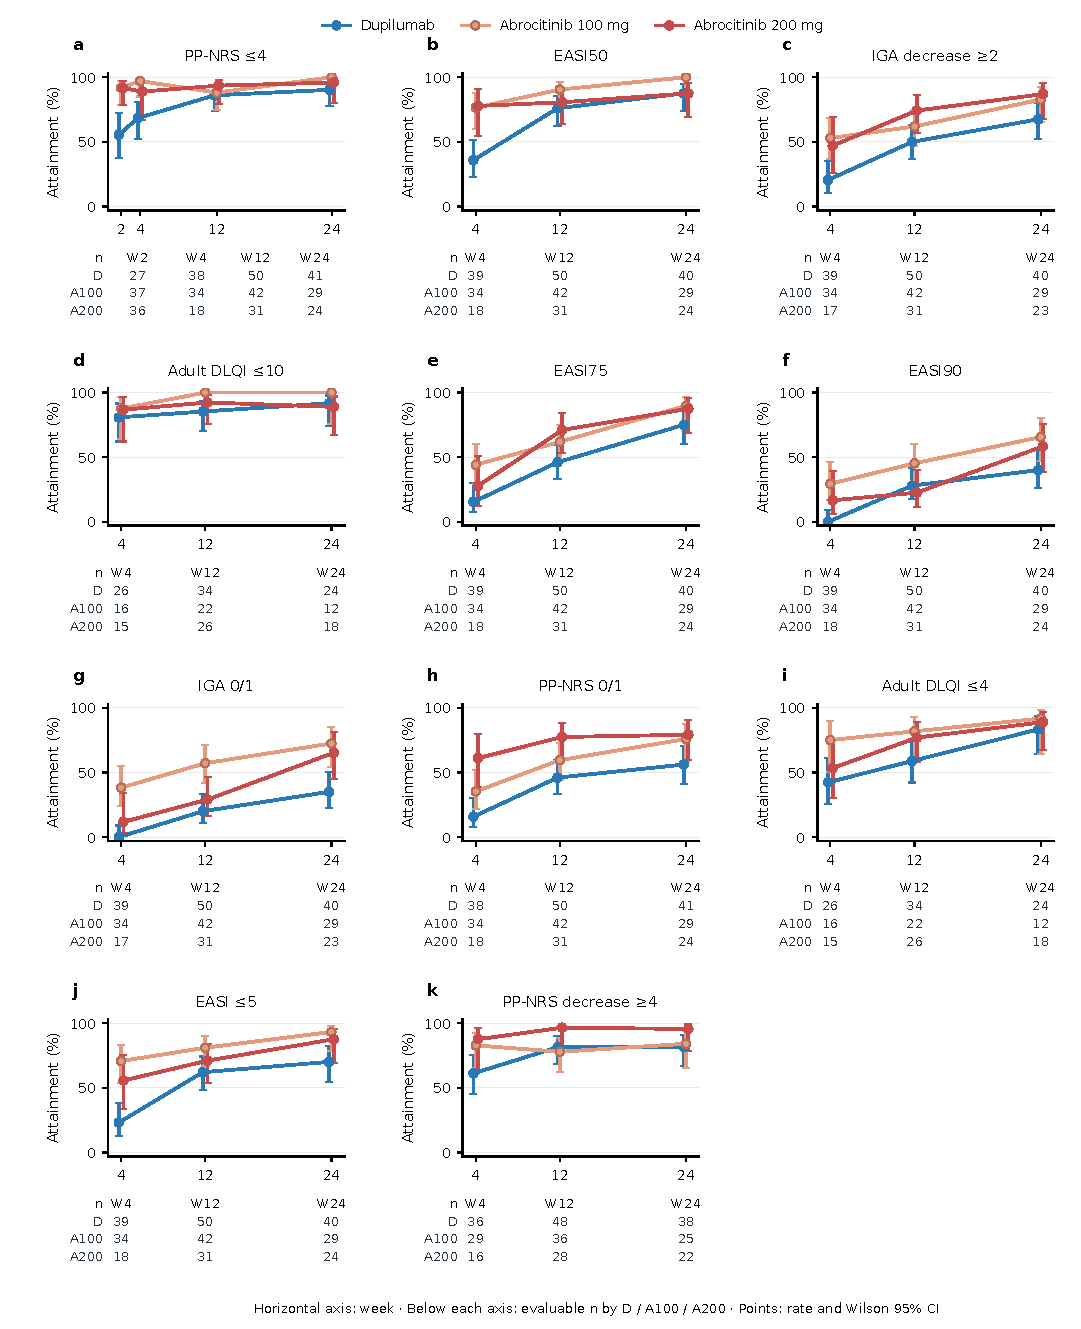
\includegraphics[width=\linewidth,height=.84\textheight,keepaspectratio]{figures/FigureS1.pdf}
\caption{\textbf{Parallel clinical and complete-input model populations.} a, Clinical comparison eligibility starts with 170 curated patients and 1,700 predefined visit slots; 736 slots contain recorded visit data. Six patients aged <12 and one age-eligible patient with an ambiguous initial dose are excluded, leaving 163 patients. This is a record source, not a screened or consented recruitment denominator. b, The linked serum branch is separate and is not a subset of the clinical comparison. Serum records count linked sample rows, not independent participants. Excluding 24 W48 records leaves 168 patients and 352 W0/W12/W24 records; age exclusions remove 12 records from six patients. Complete-case exclusions are sequential and mutually exclusive at the record level. Of the remaining 340 records, 13 lack EASI, one BSA, none CCL17, eight CCL26 and two IL-5, leaving 316 visits from 160 patients. Missing model inputs include unavailable valid positive molecular values. Losing a visit does not necessarily remove the patient. Development comprises 156 patients and 241 visits, W0 n=152 and W12 n=89. W24 comprises 75 patients and 75 visits and is previously inspected within-cohort temporal application, not external validation. The clinical and model populations share 159 patients, with four clinical-only and one model-only. Development and W24 share 71 patients, with 85 development-only and four W24-only. Fifty-one patients have all three complete model visits. Initial-dose ambiguity may remain in the treatment-free model. No missing clinical outcome is filled as validation truth. All exact counts and units remain in the linked flow and overlap source tables.}\label{fig:FigureS1}
\end{figure}
\clearpage
\renewcommand{\thefigure}{S2}
\begin{figure}[p]
\centering
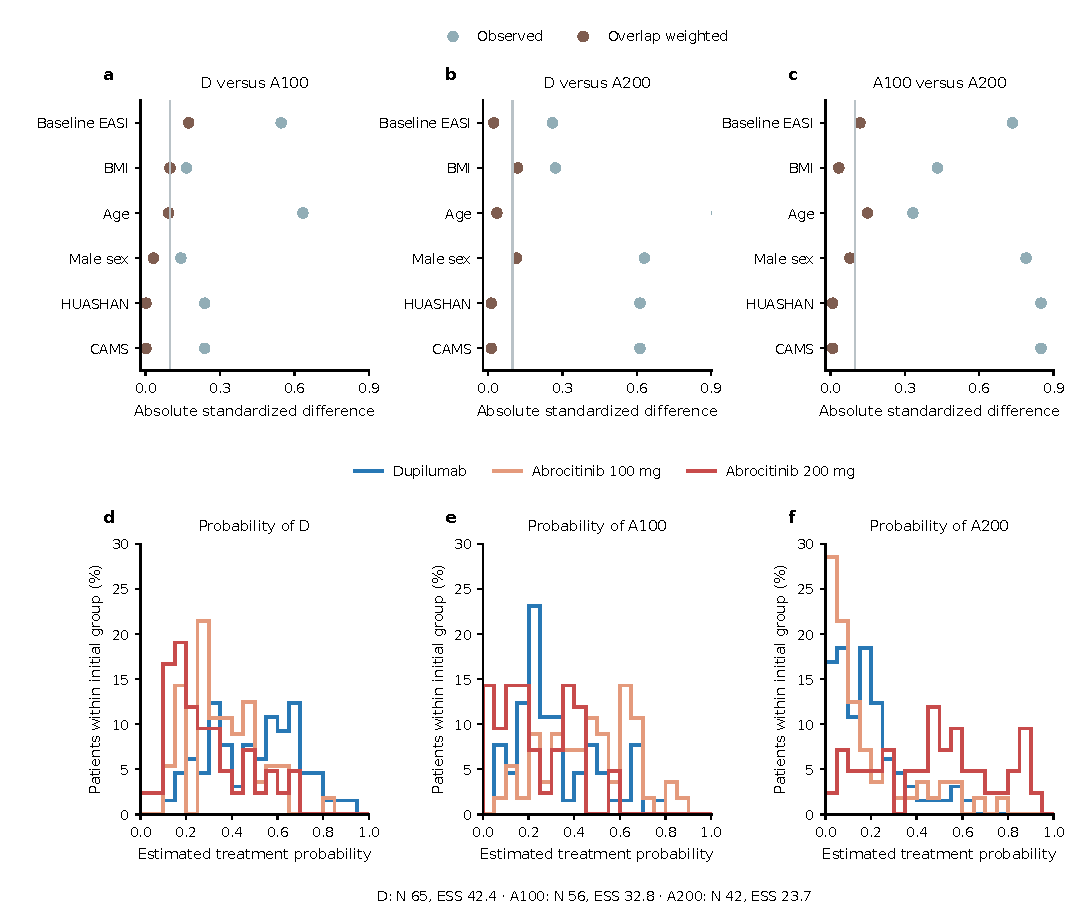
\includegraphics[width=\linewidth,height=.84\textheight,keepaspectratio]{figures/FigureS2.pdf}
\caption{\textbf{Baseline balance, treatment overlap and effective sample size.} a--c, Absolute standardized mean differences for every covariate in the initial-treatment propensity model, before and after generalized overlap weighting. Differences use the unweighted pairwise pooled standard deviation in both displays. The light 0.10 reference line is a descriptive balance guide, not a statistical significance threshold. Residual imbalance remains. d--f, Baseline multinomial treatment probabilities, stratified by actual initial treatment; each distribution uses all patients in that initial group and sums to 100\%. These show common support rather than longitudinal drug exposure. The footer reports original N and effective sample size, (sum w)$^2$/sum(w$^2$). All centre, sex, age, BMI and EASI variables are shown. Overlap weighting targets comparable baseline patients; it cannot remove unmeasured confounding or correct outcome-driven dose changes. Endpoint- and marker-specific availability/ESS diagnostics are retained in the source tables.}\label{fig:FigureS2}
\end{figure}
\clearpage
\renewcommand{\thefigure}{S3}
\begin{figure}[p]
\centering
\pdfbookmark[1]{Clinical outcomes and target comparisons}{group2}
{\large\bfseries Clinical outcomes and target comparisons}\par\vspace{5pt}
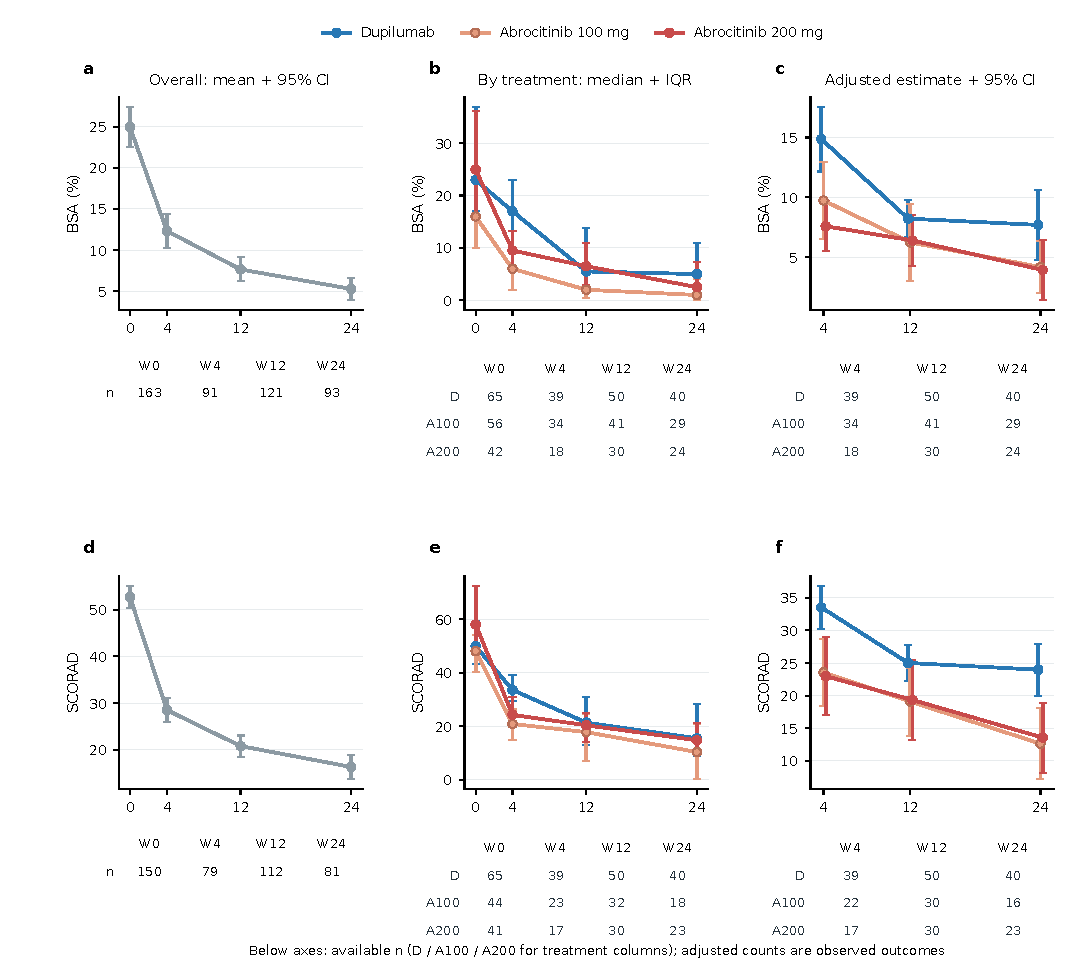
\includegraphics[width=\linewidth,height=.84\textheight,keepaspectratio]{figures/FigureS3.pdf}
\caption{\textbf{Observed and adjusted EASI, PP-NRS, Adult DLQI.} Left, observed medians with interquartile ranges by initial treatment; all available values are used at each specified visit. Right, generalized-overlap-weighted marginal estimates with patient-cluster robust 95\% confidence intervals, adjusted for baseline outcome, age, sex, BMI and centre. Patient sets can differ between visits. Exact outcome-specific counts and numerical comparisons are in the source tables; they are not replaced by a common denominator. Adult DLQI is restricted to age $\geq$18. Initial treatment groups describe observational management strategies, including subsequent regimen changes, rather than randomized fixed-dose effects.}\label{fig:FigureS3}
\end{figure}
\clearpage
\renewcommand{\thefigure}{S4}
\begin{figure}[p]
\centering
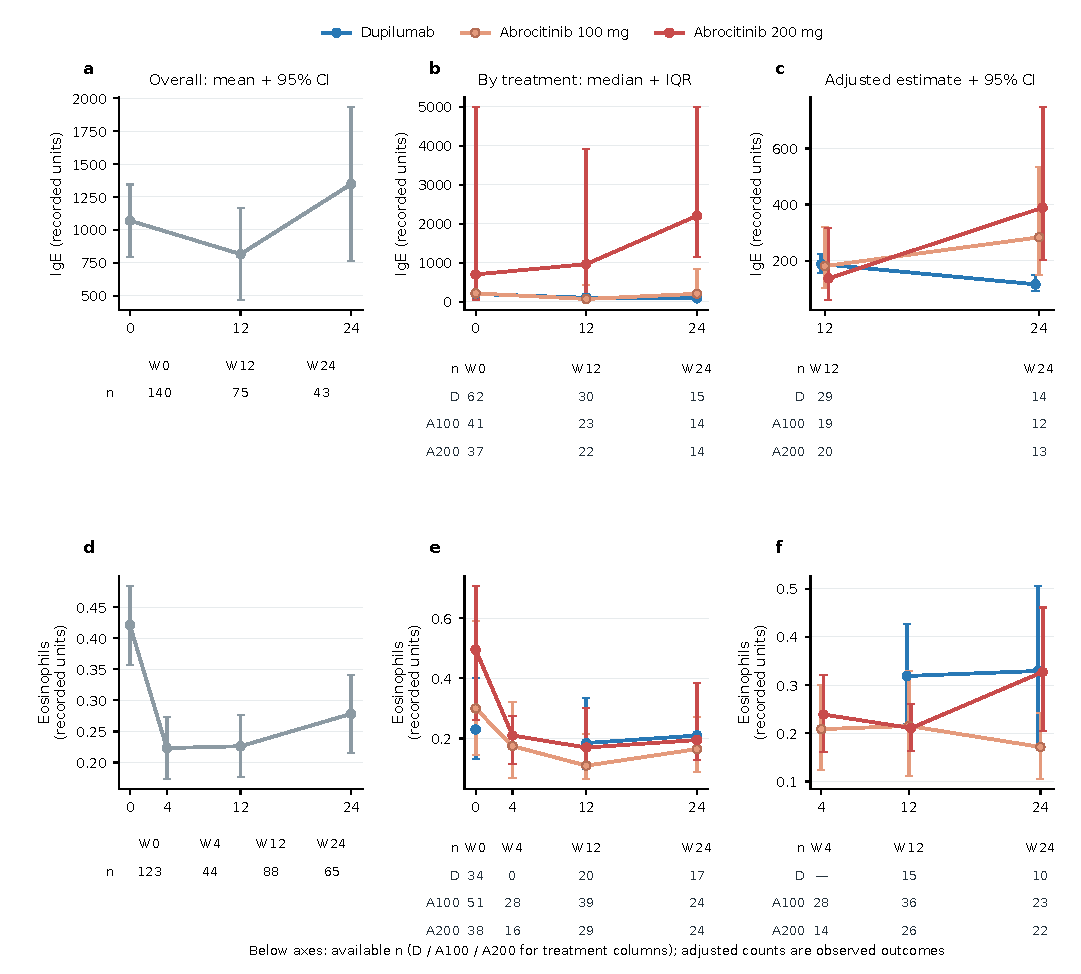
\includegraphics[width=\linewidth,height=.84\textheight,keepaspectratio]{figures/FigureS4.pdf}
\caption{\textbf{Observed and adjusted BSA (\%), SCORAD.} Left, observed medians with interquartile ranges by initial treatment; all available values are used at each specified visit. Right, generalized-overlap-weighted marginal estimates with patient-cluster robust 95\% confidence intervals, adjusted for baseline outcome, age, sex, BMI and centre. Patient sets can differ between visits. Exact outcome-specific counts and numerical comparisons are in the source tables; they are not replaced by a common denominator. Initial treatment groups describe observational management strategies, including subsequent regimen changes, rather than randomized fixed-dose effects.}\label{fig:FigureS4}
\end{figure}
\clearpage
\renewcommand{\thefigure}{S5}
\begin{figure}[p]
\centering
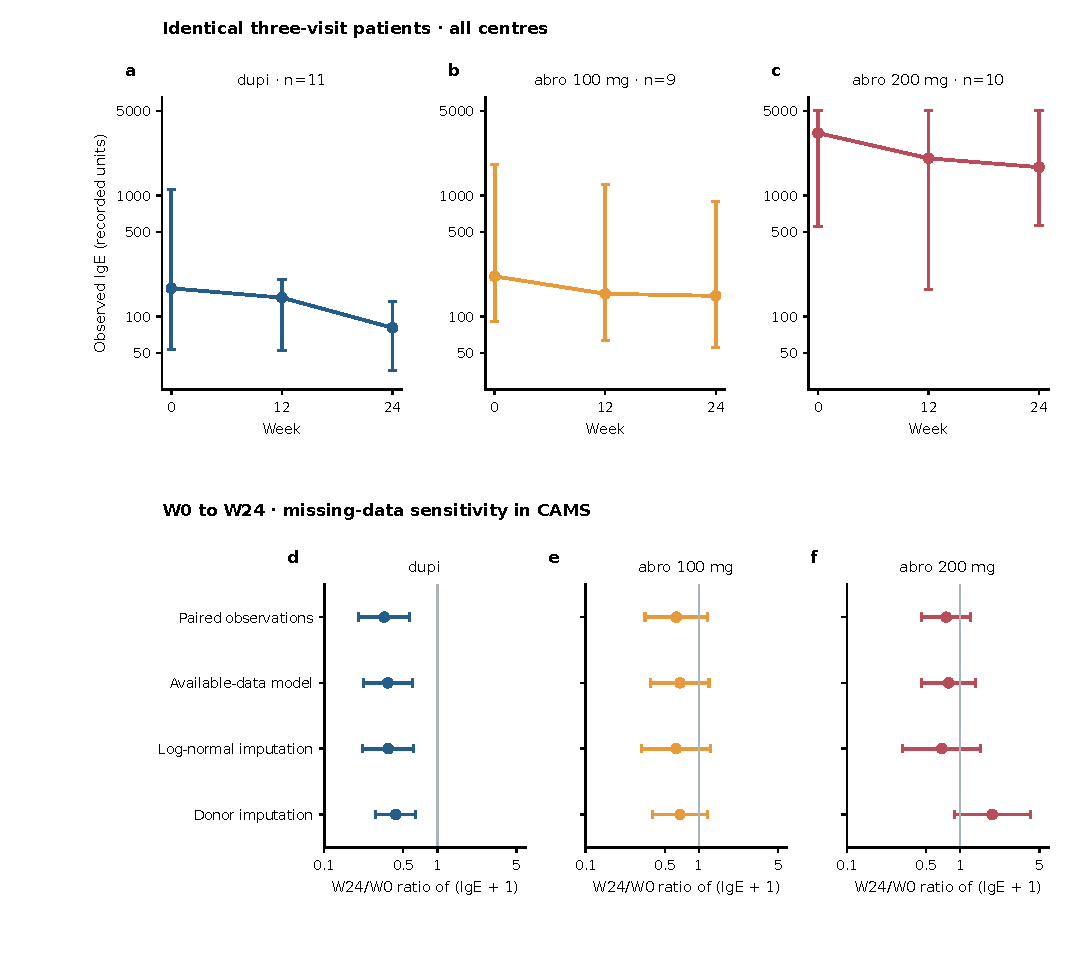
\includegraphics[width=\linewidth,height=.84\textheight,keepaspectratio]{figures/FigureS5.pdf}
\caption{\textbf{Observed and adjusted IgE (recorded units), Eosinophils (recorded units).} Left, observed medians with interquartile ranges by initial treatment; all available values are used at each specified visit. Right, generalized-overlap-weighted marginal estimates with patient-cluster robust 95\% confidence intervals, adjusted for baseline outcome, age, sex, BMI and centre. Patient sets can differ between visits. Exact outcome-specific counts and numerical comparisons are in the source tables; they are not replaced by a common denominator. IgE and eosinophils use log(1+x) models and back-transformation; adjusted estimates are not arithmetic means. IgE is shown only at W0/W12/W24. No dupilumab W4 eosinophil measurement is available; both the observed and adjusted line break at that visit. No multiple-imputation value is displayed as an observation. The separate same-patient IgE analysis tests the effect of changing sample composition. Initial treatment groups describe observational management strategies, including subsequent regimen changes, rather than randomized fixed-dose effects.}\label{fig:FigureS5}
\end{figure}
\clearpage
\renewcommand{\thefigure}{S6}
\begin{figure}[p]
\centering
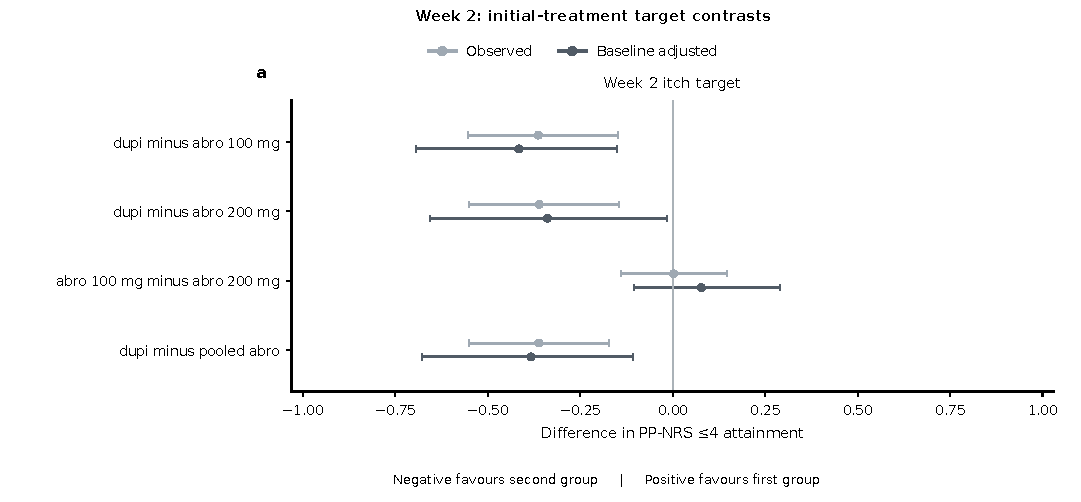
\includegraphics[width=\linewidth,height=.84\textheight,keepaspectratio]{figures/FigureS6.pdf}
\caption{\textbf{IgE with identical patients at W0, W12 and W24.} Medians and patient-bootstrap 95\% confidence intervals in fixed complete three-visit sets: 11 dupilumab, 9 A100 and 10 A200 patients. The same patients contribute at every visit within each treatment. The vertical axis is logarithmic with ticks labelled in the original recorded units; estimates and interval endpoints are unchanged. Small horizontal offsets separate treatment intervals at the same visit. No missing value is filled. These fixed-set summaries differ from available-case visit summaries and baseline-adjusted estimates because their patients and estimands differ. This check describes observation-pattern sensitivity: the small selected subsets neither estimate a causal treatment effect nor establish arithmetic mean changes. Laboratory units require source confirmation.}\label{fig:FigureS6}
\end{figure}
\clearpage
\renewcommand{\thefigure}{S7}
\begin{figure}[p]
\centering
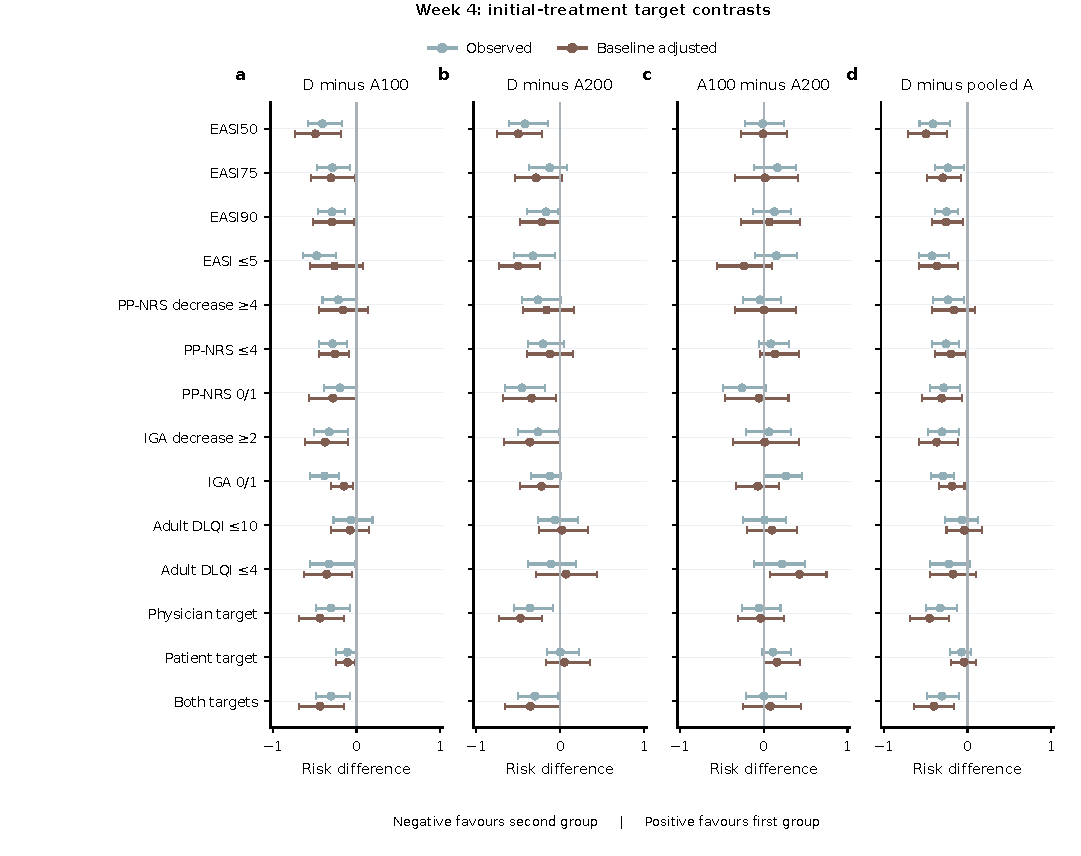
\includegraphics[width=\linewidth,height=.84\textheight,keepaspectratio]{figures/FigureS7.pdf}
\caption{\textbf{Week 2: all initial-treatment target contrasts.} Observed and baseline-adjusted risk differences with nominal 95\% confidence intervals. Positive values favour the first named treatment for target attainment. Adjustment uses generalized overlap weights from baseline EASI, age, sex, BMI and centre; it does not estimate a randomized current-dose effect. D denotes dupilumab; A100/A200 the initial abrocitinib doses. Pooled abrocitinib is supplementary. Missing estimates are left absent; all exact denominators, Fisher/weighted tests, Holm-adjusted P values and exploratory FDR values are in the source tables.}\label{fig:FigureS7}
\end{figure}
\clearpage
\renewcommand{\thefigure}{S8}
\begin{figure}[p]
\centering
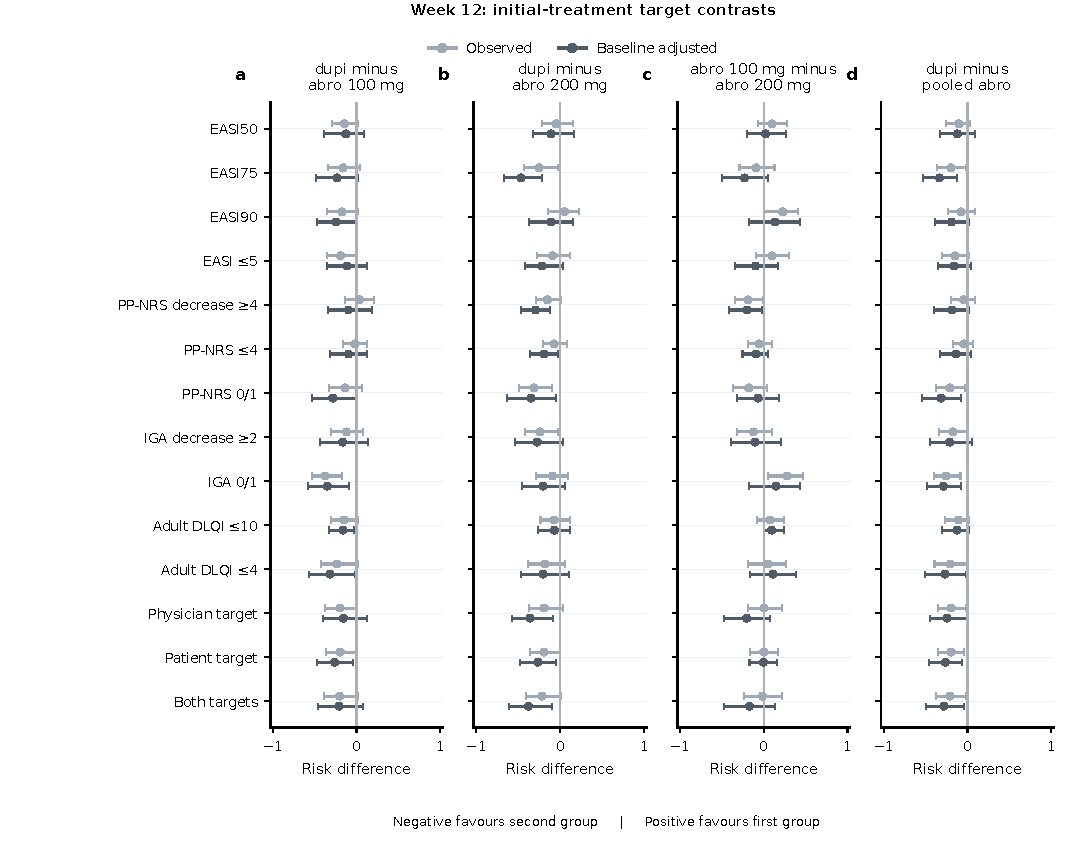
\includegraphics[width=\linewidth,height=.84\textheight,keepaspectratio]{figures/FigureS8.pdf}
\caption{\textbf{Week 4: all initial-treatment target contrasts.} Observed and baseline-adjusted risk differences with nominal 95\% confidence intervals. Positive values favour the first named treatment for target attainment. Adjustment uses generalized overlap weights from baseline EASI, age, sex, BMI and centre; it does not estimate a randomized current-dose effect. D denotes dupilumab; A100/A200 the initial abrocitinib doses. Pooled abrocitinib is supplementary. Missing estimates are left absent; all exact denominators, Fisher/weighted tests, Holm-adjusted P values and exploratory FDR values are in the source tables.}\label{fig:FigureS8}
\end{figure}
\clearpage
\renewcommand{\thefigure}{S9}
\begin{figure}[p]
\centering
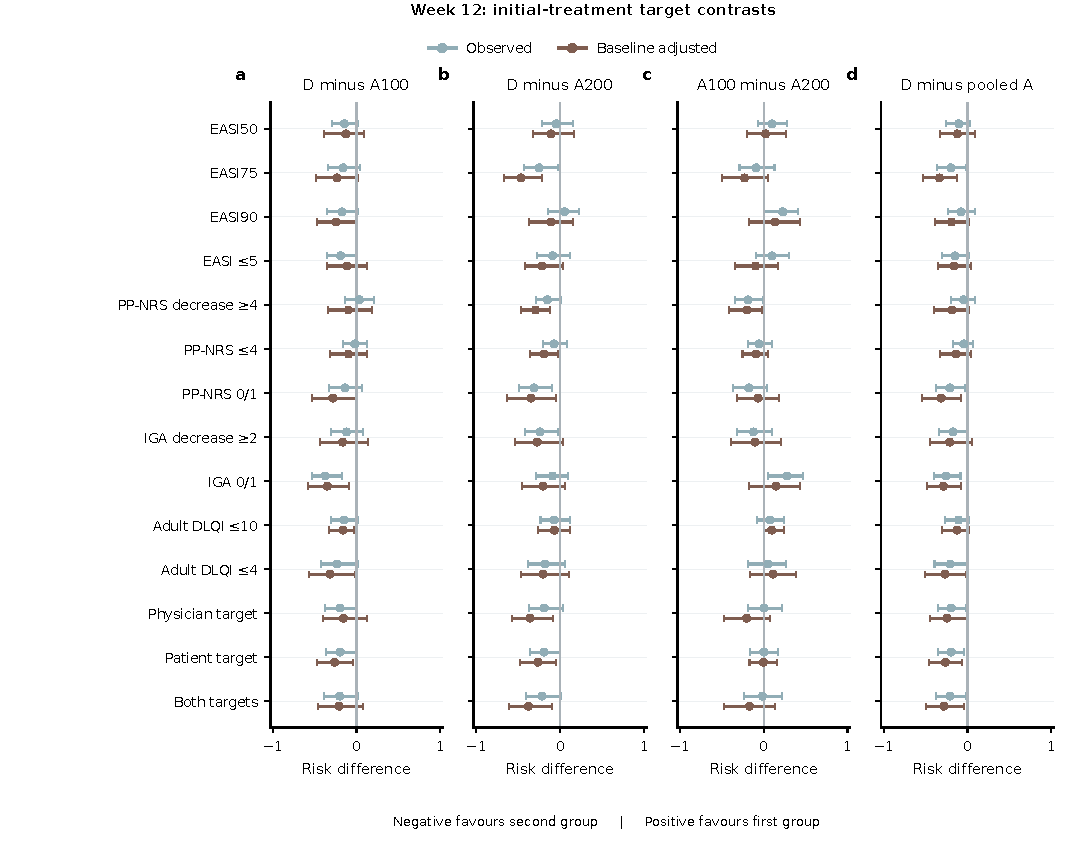
\includegraphics[width=\linewidth,height=.84\textheight,keepaspectratio]{figures/FigureS9.pdf}
\caption{\textbf{Week 12: all initial-treatment target contrasts.} Observed and baseline-adjusted risk differences with nominal 95\% confidence intervals. Positive values favour the first named treatment for target attainment. Adjustment uses generalized overlap weights from baseline EASI, age, sex, BMI and centre; it does not estimate a randomized current-dose effect. D denotes dupilumab; A100/A200 the initial abrocitinib doses. Pooled abrocitinib is supplementary. Missing estimates are left absent; all exact denominators, Fisher/weighted tests, Holm-adjusted P values and exploratory FDR values are in the source tables.}\label{fig:FigureS9}
\end{figure}
\clearpage
\renewcommand{\thefigure}{S10}
\begin{figure}[p]
\centering
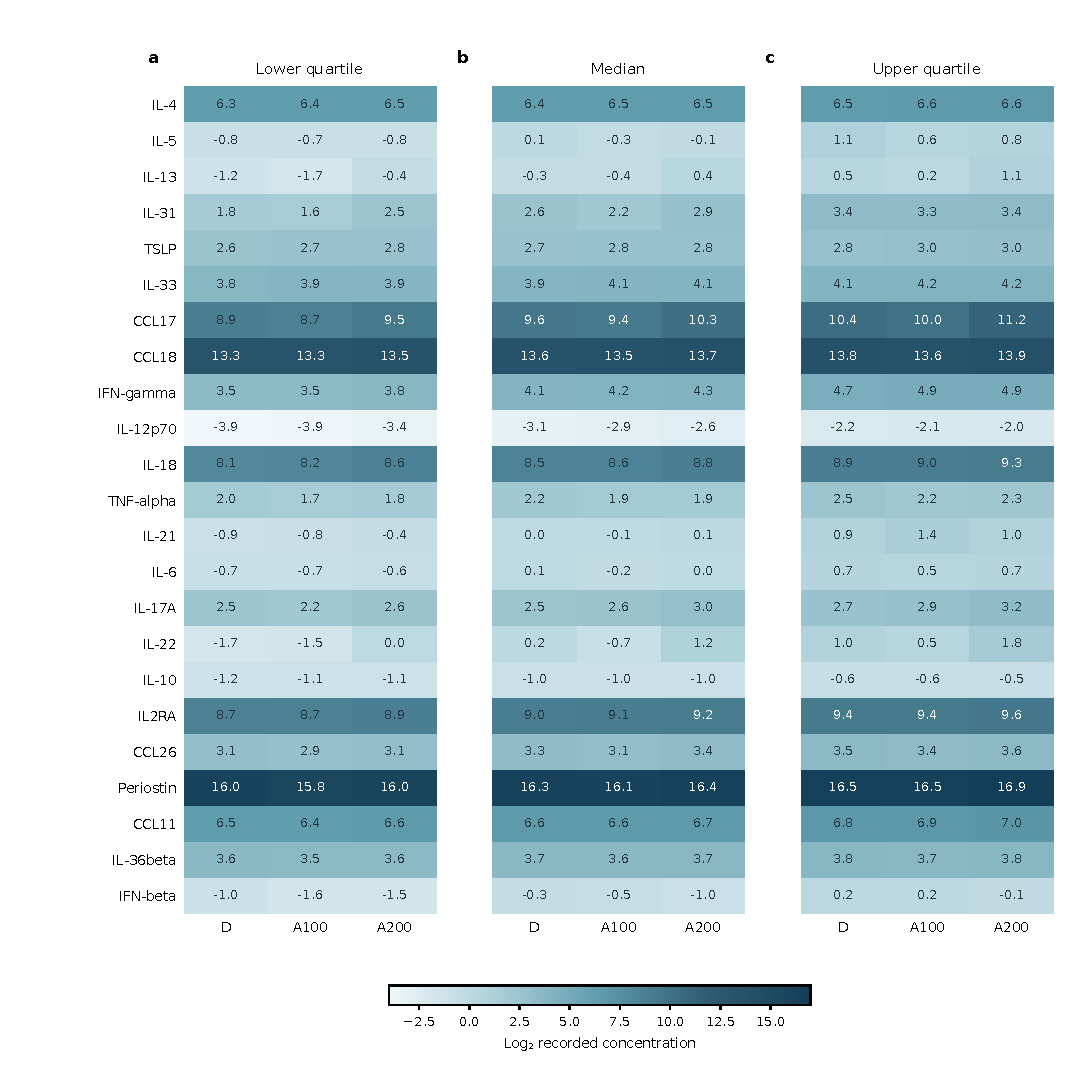
\includegraphics[width=\linewidth,height=.84\textheight,keepaspectratio]{figures/FigureS10.pdf}
\caption{\textbf{Week 24: all initial-treatment target contrasts.} Observed and baseline-adjusted risk differences with nominal 95\% confidence intervals. Positive values favour the first named treatment for target attainment. Adjustment uses generalized overlap weights from baseline EASI, age, sex, BMI and centre; it does not estimate a randomized current-dose effect. D denotes dupilumab; A100/A200 the initial abrocitinib doses. Pooled abrocitinib is supplementary. Missing estimates are left absent; all exact denominators, Fisher/weighted tests, Holm-adjusted P values and exploratory FDR values are in the source tables.}\label{fig:FigureS10}
\end{figure}
\clearpage
\renewcommand{\thefigure}{S11}
\begin{figure}[p]
\centering
\pdfbookmark[1]{Serum changes and regional disease}{group3}
{\large\bfseries Serum changes and regional disease}\par\vspace{5pt}
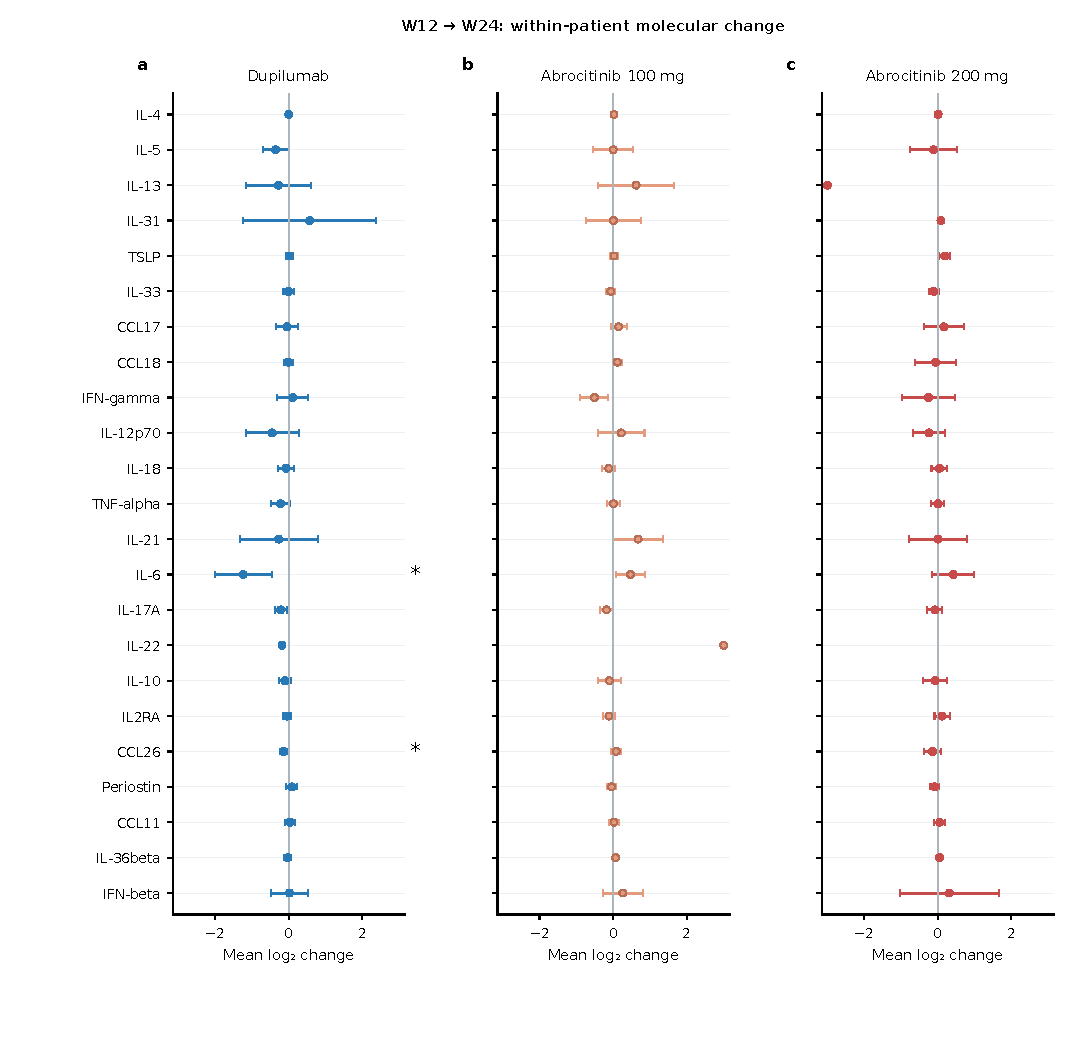
\includegraphics[width=\linewidth,height=.84\textheight,keepaspectratio]{figures/FigureS11.pdf}
\caption{\textbf{Baseline distributions of all 23 serum markers.} Cells display the lower quartile, median and upper quartile of baseline log$_2$ recorded concentration for each initial treatment. All three panels use the same numeric colour scale without row normalization. Compare treatments within a marker: concentration differences between distinct analytes do not indicate differences in biological activity. D denotes dupilumab; A100/A200 initial abrocitinib 100/200 mg. Every measured marker is retained. The source table includes exact counts, censoring-related availability, ranges and distribution summaries; quartiles summarize available positive numeric observations and do not replace censored values.}\label{fig:FigureS11}
\end{figure}
\clearpage
\renewcommand{\thefigure}{S12}
\begin{figure}[p]
\centering
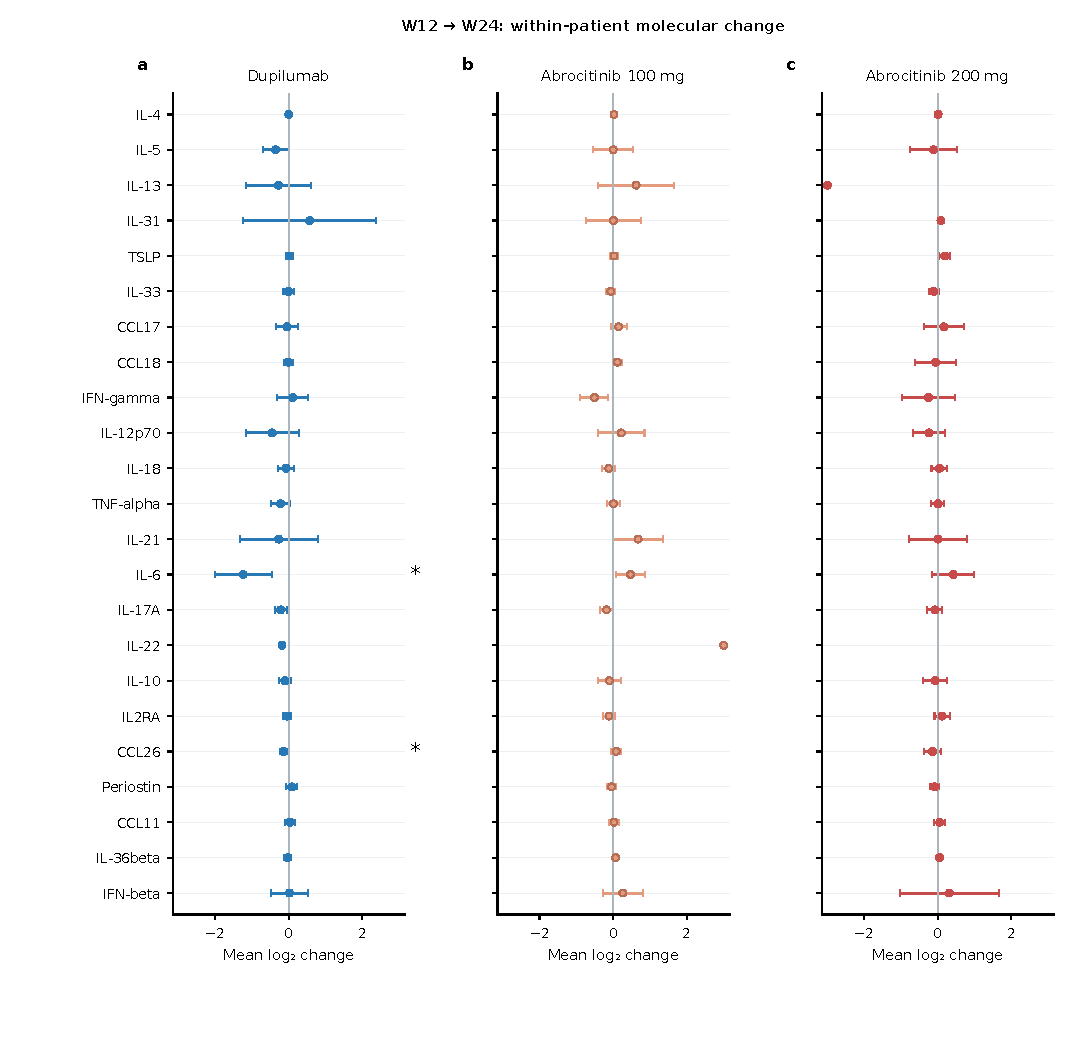
\includegraphics[width=\linewidth,height=.84\textheight,keepaspectratio]{figures/FigureS12.pdf}
\caption{\textbf{Molecular changes from W12 to W24.} Mean paired log$_2$ concentration changes with 95\% t confidence intervals. Negative values indicate lower later concentration. Each marker/treatment uses all available pairs for this interval; exact counts are in the source table. All 23 measured markers are retained. Estimates based on fewer than five pairs are descriptive and have no inferential interval; unavailable estimates are blank. Stars denote BH q<0.05 across the full 207 marker-by-treatment-by-window family, not a separate family for the displayed interval.}\label{fig:FigureS12}
\end{figure}
\clearpage
\renewcommand{\thefigure}{S13}
\begin{figure}[p]
\centering
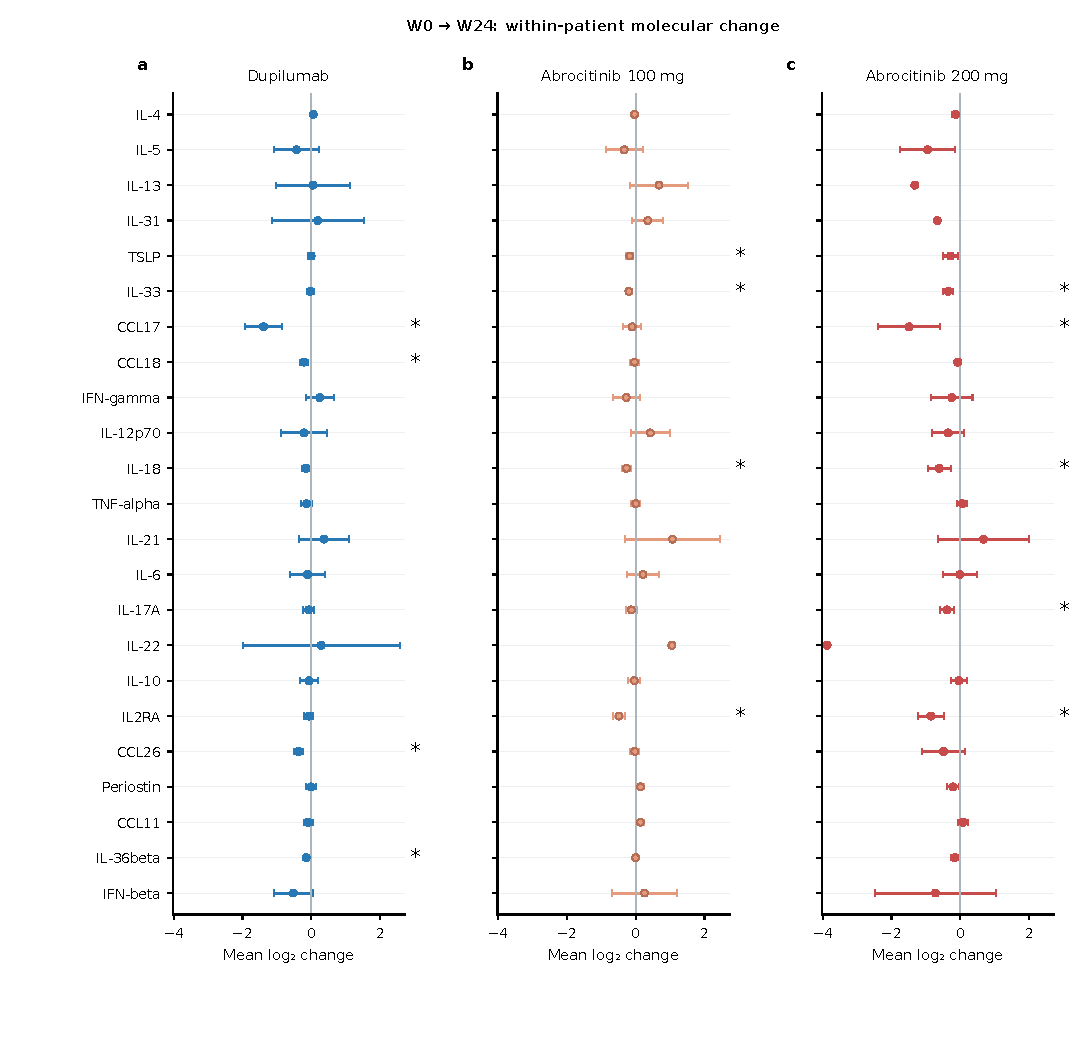
\includegraphics[width=\linewidth,height=.84\textheight,keepaspectratio]{figures/FigureS13.pdf}
\caption{\textbf{Molecular changes from W0 to W24.} Mean paired log$_2$ concentration changes with 95\% t confidence intervals. Negative values indicate lower later concentration. Each marker/treatment uses all available pairs for this interval; exact counts are in the source table. All 23 measured markers are retained. Estimates based on fewer than five pairs are descriptive and have no inferential interval; unavailable estimates are blank. Stars denote BH q<0.05 across the full 207 marker-by-treatment-by-window family, not a separate family for the displayed interval.}\label{fig:FigureS13}
\end{figure}
\clearpage
\renewcommand{\thefigure}{S14}
\begin{figure}[p]
\centering
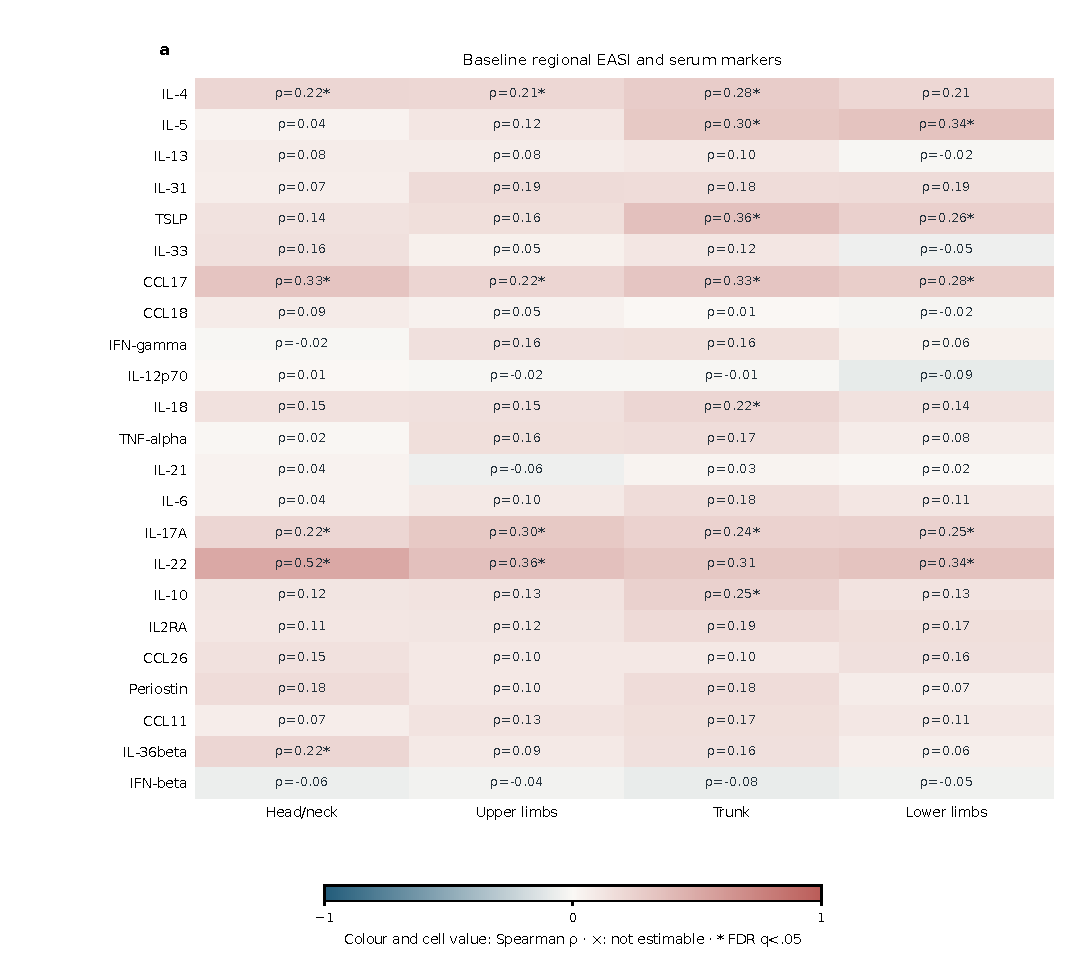
\includegraphics[width=\linewidth,height=.84\textheight,keepaspectratio]{figures/FigureS14.pdf}
\caption{\textbf{Adjusted molecular comparisons from W0 to W12.} Differences in within-patient log$_2$ changes with HC3 95\% confidence intervals. Negative values mean a smaller, more negative change in the first named treatment. Models adjust starting log$_2$ concentration, baseline total EASI, age, sex, BMI and centre. D, dupilumab; A100/A200, initial abrocitinib 100/200 mg. Pooled A retains the observed dose mixture. Stars denote the original BH q<0.05 family; no multiplicity family is recalculated after display selection. Blank positions have no estimable contrast. Complete counts, diagnostics, centre/batch sensitivities and tests remain in the source table. The W0--W12 D-minus-pooled-A and A200-minus-A100 comparisons are in the main molecular figure. These are adjusted observational associations, not randomized current-dose effects.}\label{fig:FigureS14}
\end{figure}
\clearpage
\renewcommand{\thefigure}{S15}
\begin{figure}[p]
\centering
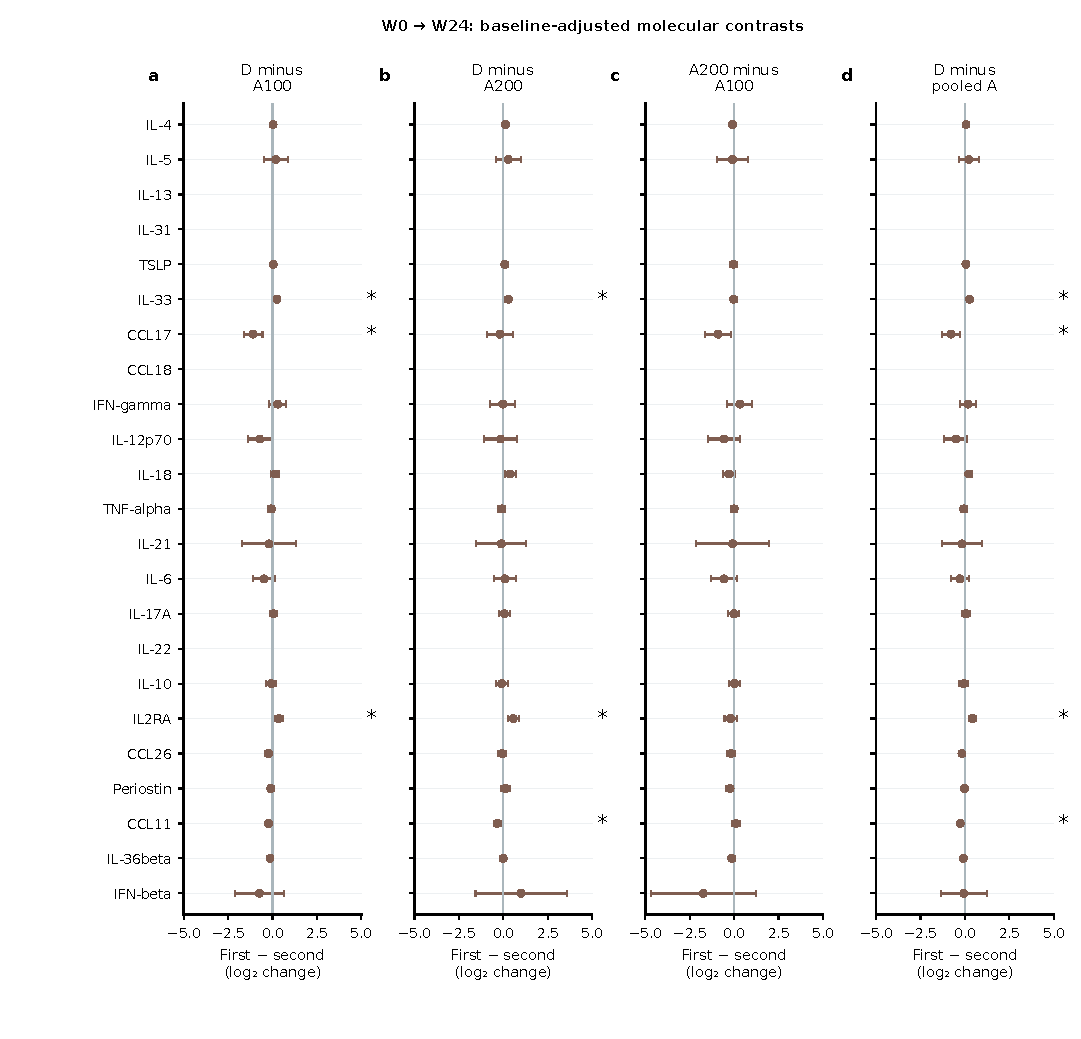
\includegraphics[width=\linewidth,height=.84\textheight,keepaspectratio]{figures/FigureS15.pdf}
\caption{\textbf{Adjusted molecular comparisons from W12 to W24.} Differences in within-patient log$_2$ changes with HC3 95\% confidence intervals. Negative values mean a smaller, more negative change in the first named treatment. Models adjust starting log$_2$ concentration, baseline total EASI, age, sex, BMI and centre. D, dupilumab; A100/A200, initial abrocitinib 100/200 mg. Pooled A retains the observed dose mixture. Stars denote the original BH q<0.05 family; no multiplicity family is recalculated after display selection. Blank positions have no estimable contrast. Complete counts, diagnostics, centre/batch sensitivities and tests remain in the source table. These are adjusted observational associations, not randomized current-dose effects.}\label{fig:FigureS15}
\end{figure}
\clearpage
\renewcommand{\thefigure}{S16}
\begin{figure}[p]
\centering
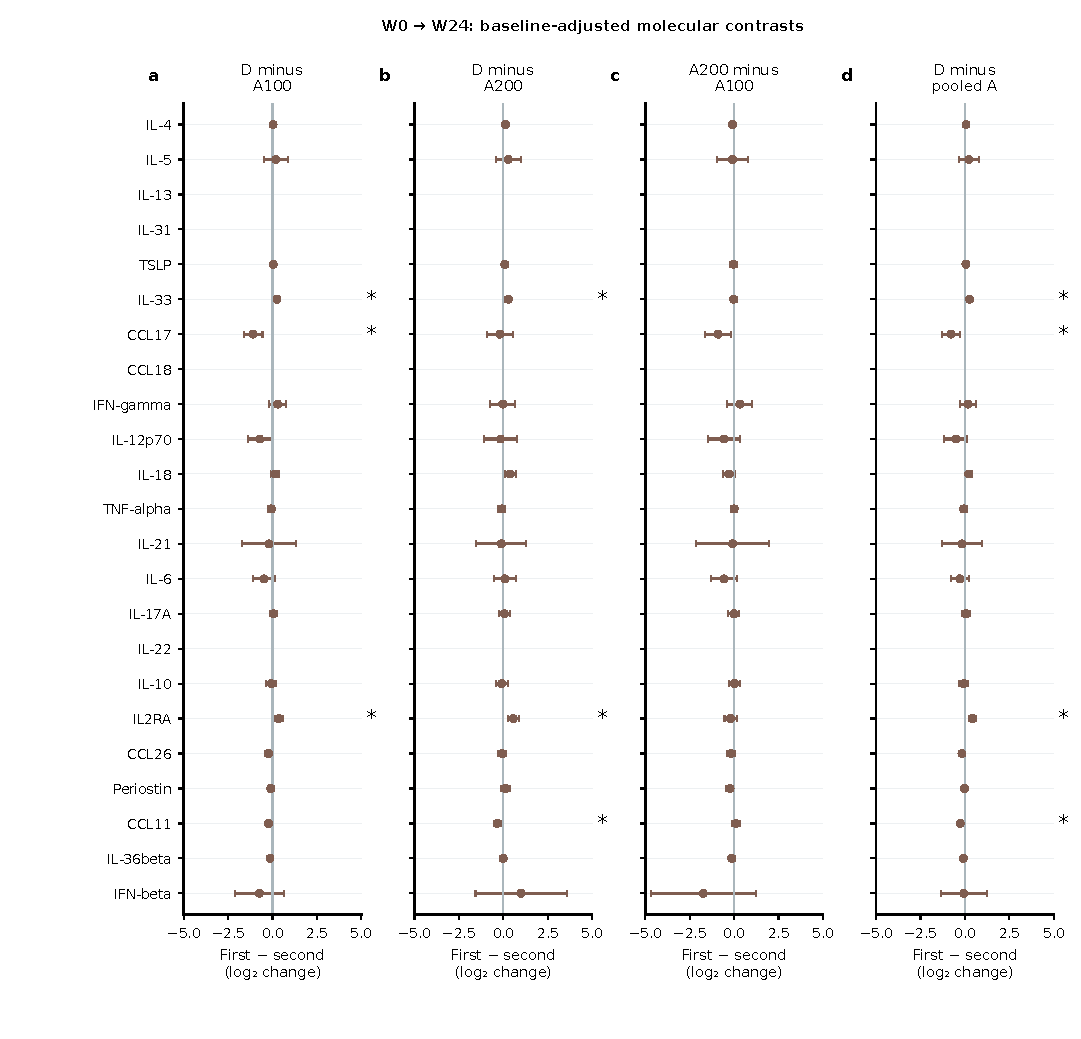
\includegraphics[width=\linewidth,height=.84\textheight,keepaspectratio]{figures/FigureS16.pdf}
\caption{\textbf{Adjusted molecular comparisons from W0 to W24.} Differences in within-patient log$_2$ changes with HC3 95\% confidence intervals. Negative values mean a smaller, more negative change in the first named treatment. Models adjust starting log$_2$ concentration, baseline total EASI, age, sex, BMI and centre. D, dupilumab; A100/A200, initial abrocitinib 100/200 mg. Pooled A retains the observed dose mixture. Stars denote the original BH q<0.05 family; no multiplicity family is recalculated after display selection. Blank positions have no estimable contrast. Complete counts, diagnostics, centre/batch sensitivities and tests remain in the source table. These are adjusted observational associations, not randomized current-dose effects.}\label{fig:FigureS16}
\end{figure}
\clearpage
\renewcommand{\thefigure}{S17}
\begin{figure}[p]
\centering
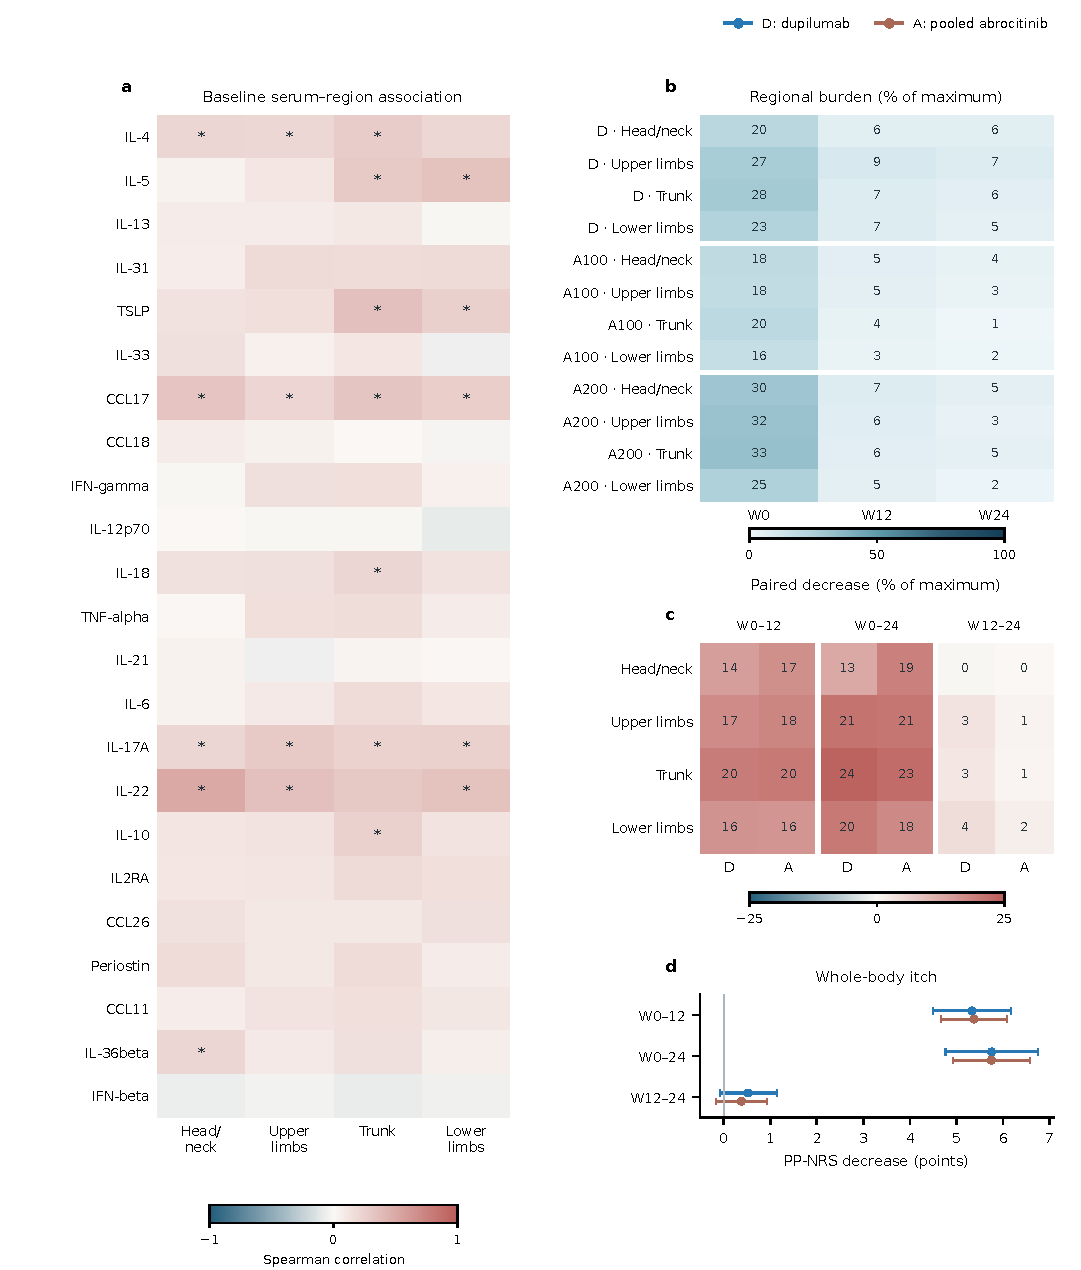
\includegraphics[width=\linewidth,height=.84\textheight,keepaspectratio]{figures/FigureS17.pdf}
\caption{\textbf{Molecular and clinical changes associated after multiplicity correction.} Every association meeting BH q<0.05 in the full declared change-association family is displayed; selection spans 23 markers, five clinical outcomes, three initial treatments and three intervals. No W12--W24 association met this threshold. Points are Spearman correlations between within-patient clinical change and log$_2$ molecular change, both later minus earlier, with patient-bootstrap 95\% confidence intervals. Positive correlations indicate changes in the same direction. Labels give paired-patient counts and the interval; colours indicate initial treatment only. Adult DLQI requires age $\geq$18. All tested coefficients, non-significant results and unestimable pairs remain in the complete source table. This significance-selected display is exploratory and is not independent validation, numerical agreement or a causal molecular effect.}\label{fig:FigureS17}
\end{figure}
\clearpage
\renewcommand{\thefigure}{S18}
\begin{figure}[p]
\centering
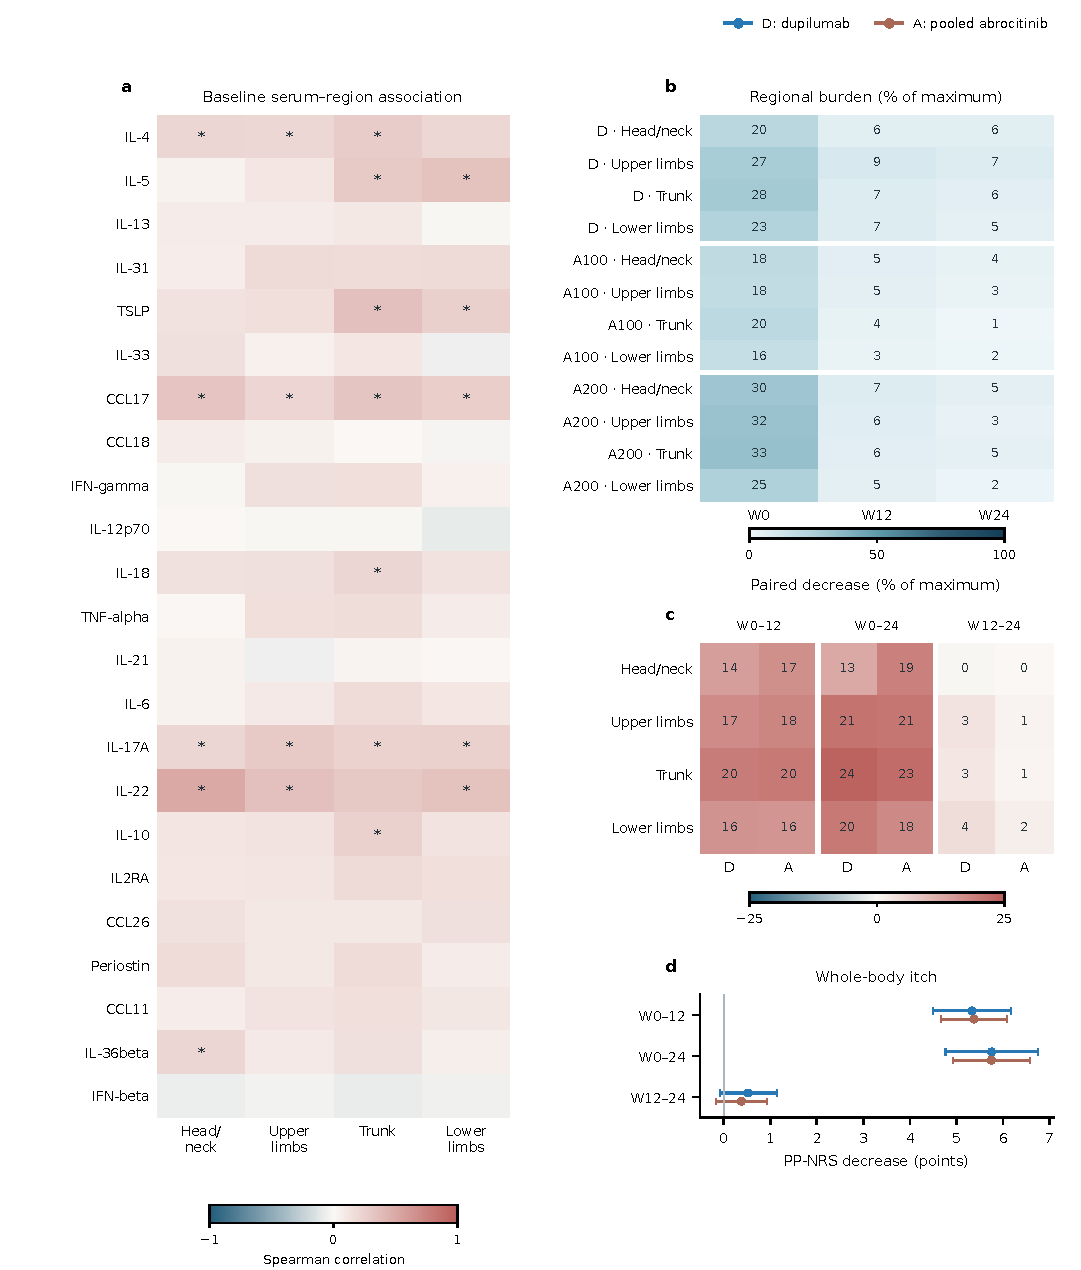
\includegraphics[width=\linewidth,height=.84\textheight,keepaspectratio]{figures/FigureS18.pdf}
\caption{\textbf{Regional clinical burden and molecular associations.} a, Baseline Spearman associations between all 23 markers and the four regional EASI contributions; stars mark BH q<0.05, with complete coefficients, patient counts and bootstrap intervals retained in the source. b, Available-case mean regional EASI divided by its theoretical maximum and multiplied by 100; cells show percentages, not patient counts. c, Mean paired regional decrease as a percentage of the same regional maximum for three separately labelled intervals; positive values indicate improvement. D is dupilumab and A is the observed pooled abrocitinib dose mixture. These heatmaps summarize magnitude; exact 95\% t intervals and counts are in the source tables. d, Whole-body PP-NRS mean decreases with 95\% t intervals, not region-specific itch. Regional maxima are 7.2, 14.4, 21.6 and 28.8 for head/neck, upper limbs, trunk and lower limbs. All regional analyses require complete, bounded regional records consistent with total EASI. Intervals can share patients and are not successive cumulative effects. Colour bars encode distinct quantities and are not interchangeable. No baseline-adjusted regional treatment contrast passed the FDR threshold; full separate-dose comparisons remain available.}\label{fig:FigureS18}
\end{figure}
\clearpage
\renewcommand{\thefigure}{S19}
\begin{figure}[p]
\centering
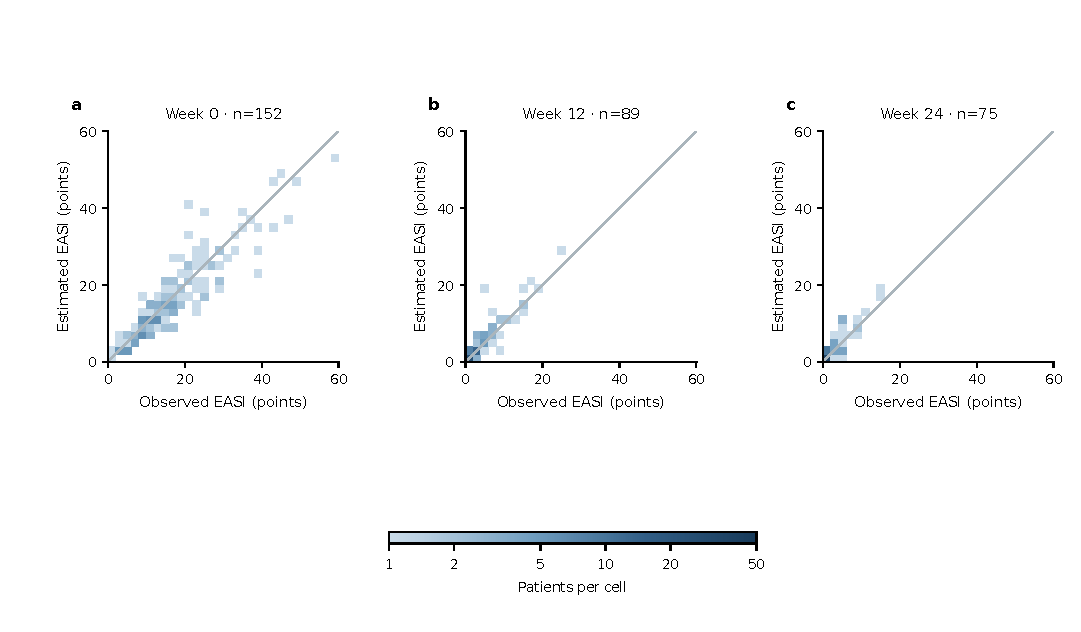
\includegraphics[width=\linewidth,height=.84\textheight,keepaspectratio]{figures/FigureS19.pdf}
\caption{\textbf{Three-visit molecular trajectories in fixed patient sets.} Within each marker and treatment, the same patients contribute at W0, W12 and W24. W0 is zero by definition; W12/W24 are mean within-patient log$_2$ changes from W0. Light blue, teal and deep blue encode W0/W12/W24 consistently across all panels. Rows are spaced to separate the three visits; horizontal intervals are 95\% t confidence intervals for n$\geq$5. Smaller sets are descriptive without inferential intervals, and absent estimates remain blank. All 23 markers are retained. Fixed triplet counts are available in the source table and may differ across markers or treatments, but never across the three displayed visits within a marker/treatment.}\label{fig:FigureS19}
\end{figure}
\clearpage
\renewcommand{\thefigure}{S20}
\begin{figure}[p]
\centering
\pdfbookmark[1]{Individual EASI estimation and monitoring}{group4}
{\large\bfseries Individual EASI estimation and monitoring}\par\vspace{5pt}
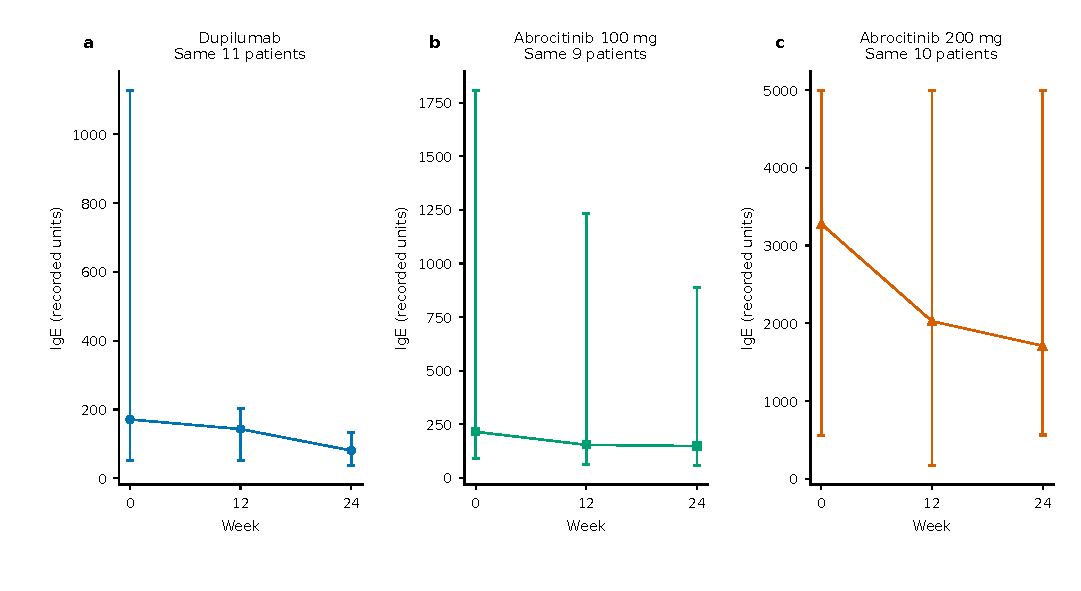
\includegraphics[width=\linewidth,height=.84\textheight,keepaspectratio]{figures/FigureS20.pdf}
\caption{\textbf{Individual EASI estimation and its severity boundary.} a--c, Estimated versus observed EASI in the first patient-held-out repetition at W0/W12 and same-cohort temporal application at W24. Each fixed 2$\times$2-EASI-point cell contains all patients whose exact score pair falls within its boundaries. Colour gives patient count on the shared logarithmic count scale; white cells have no observations. All 152/89/75 eligible patients are retained, and identical axes preserve the severity-range comparison. Grey lines denote exact agreement, not a fitted association. d, Cumulative absolute-error proportions, calculated separately in each validation repetition and then averaged. Bands are patient-bootstrap 95\% confidence intervals conditional on saved predictions. All errors enter each proportion; only thresholds from zero to ten points are displayed. The two-point line is a reading reference, not an accepted replacement margin. e, Baseline MAE by observed EASI stratum, with patient-bootstrap 95\% confidence intervals and unique-patient counts. These estimates average the two repetition-specific metrics. W12/W24 have only one/no EASI>21 observation, respectively. W0/W12 use nested patient-level structure and penalty selection; earlier marker selection is not repeated. W24 was previously inspected within the same cohort. These results assess the development procedure, not independent validation of the final formula. Primary overall metrics and numerical controls appear in Table 2; molecular added accuracy has not been established.}\label{fig:FigureS20}
\end{figure}
\clearpage
\renewcommand{\thefigure}{S21}
\begin{figure}[p]
\centering
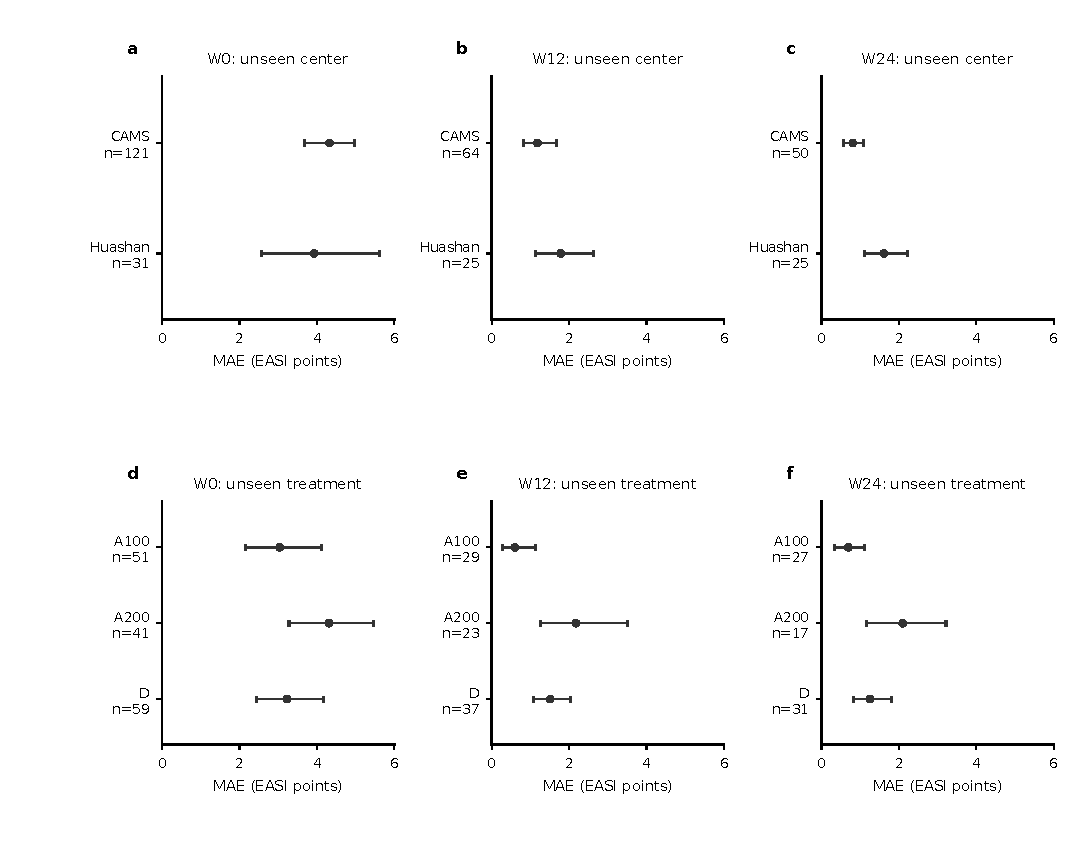
\includegraphics[width=\linewidth,height=.84\textheight,keepaspectratio]{figures/FigureS21.pdf}
\caption{\textbf{Within-patient change and EASI75 response classification.} a--c, Estimated versus observed EASI changes in the first patient-held-out repetition. Change is end minus start, so negative values indicate improvement. Fixed 2$\times$2-EASI-point cells count exact paired score changes, using one logarithmic count scale and identical axes across intervals; white cells contain no observations. All 85, 67 and 55 paired patients are retained in their respective windows, which can share patients. Grey diagonal lines denote exact agreement; horizontal and vertical lines mark no change. Primary change MAEs over W0--W12, W0--W24 and W12--W24 are 3.87, 3.47 and 1.49 points, respectively, with intervals in the source tables. These metrics score each of two repetitions before averaging, whereas the count maps illustrate one repetition. d, EASI75 sensitivity, specificity and overall agreement, averaged after classification within each repetition, with patient-bootstrap 95\% confidence intervals conditional on saved predictions. Sensitivity denominators are observed responders (W12 n=49; W24 n=54); specificity denominators are nonresponders (36 and 13). Agreement includes 85 and 67 patients. Observed and estimated response each use their corresponding W0 and follow-up scores; percentage response requires positive observed and estimated W0. W24 is previously inspected same-cohort temporal application, not external validation. Complete EASI50/75/90 classifications and exclusions remain in the supplement. These results assess monitoring agreement, not treatment causality or clinical interchangeability.}\label{fig:FigureS21}
\end{figure}
\clearpage
\renewcommand{\thefigure}{S22}
\begin{figure}[p]
\centering
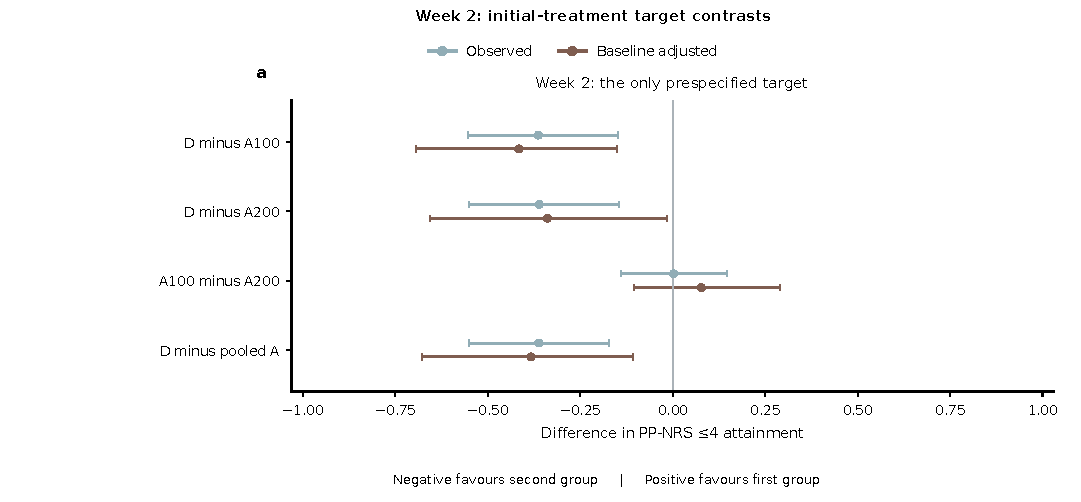
\includegraphics[width=\linewidth,height=.84\textheight,keepaspectratio]{figures/FigureS22.pdf}
\caption{\textbf{Who is correctly classified as reaching EASI50, EASI75 and EASI90?.} Each panel shows actual patient counts from the first outer repetition, separately for W0$\rightarrow$W12 and W0$\rightarrow$W24. Rows are observed response and columns model-estimated response. Diagonal cells are correct; upper-right cells falsely indicate response and lower-left cells miss an observed responder. Percentages are within each observed-response row, so the lower-right percentage is sensitivity and the upper-left percentage specificity. Observed response uses observed baseline/follow-up scores, whereas estimated response uses predicted baseline/follow-up scores. Counts are integers from one repetition, not the primary two-repetition average; the full metrics table retains the latter. The paired denominators are 85 and 67, with no excluded pair for invalid baseline in this displayed repetition. The two intervals can share patients. This assesses response classification, not alternative-treatment outcomes or continuous-score equivalence.}\label{fig:FigureS22}
\end{figure}
\clearpage\section*{Aggregate source tables}
The \href{run:source_data/index.csv}{machine-readable source-table index} lists the complete aggregate collection, including unplotted and negative results. Figure-specific dependencies are in \texttt{figure\_catalog.json}. The \href{https://github.com/yanax726/T2T/tree/main/results/tables/update_20261017}{versioned aggregate directory} includes clinical, molecular, model, regional and reference-sensitivity tables; restricted patient-level files are not part of the public collection.
\bibliographystyle{unsrtnat}\bibliography{references}
\end{document}
